% Options for packages loaded elsewhere
\PassOptionsToPackage{unicode}{hyperref}
\PassOptionsToPackage{hyphens}{url}
\PassOptionsToPackage{dvipsnames,svgnames,x11names}{xcolor}
%
\documentclass[
  letterpaper,
  DIV=11,
  numbers=noendperiod]{scrreprt}

\usepackage{amsmath,amssymb}
\usepackage{iftex}
\ifPDFTeX
  \usepackage[T1]{fontenc}
  \usepackage[utf8]{inputenc}
  \usepackage{textcomp} % provide euro and other symbols
\else % if luatex or xetex
  \usepackage{unicode-math}
  \defaultfontfeatures{Scale=MatchLowercase}
  \defaultfontfeatures[\rmfamily]{Ligatures=TeX,Scale=1}
\fi
\usepackage{lmodern}
\ifPDFTeX\else  
    % xetex/luatex font selection
\fi
% Use upquote if available, for straight quotes in verbatim environments
\IfFileExists{upquote.sty}{\usepackage{upquote}}{}
\IfFileExists{microtype.sty}{% use microtype if available
  \usepackage[]{microtype}
  \UseMicrotypeSet[protrusion]{basicmath} % disable protrusion for tt fonts
}{}
\makeatletter
\@ifundefined{KOMAClassName}{% if non-KOMA class
  \IfFileExists{parskip.sty}{%
    \usepackage{parskip}
  }{% else
    \setlength{\parindent}{0pt}
    \setlength{\parskip}{6pt plus 2pt minus 1pt}}
}{% if KOMA class
  \KOMAoptions{parskip=half}}
\makeatother
\usepackage{xcolor}
\setlength{\emergencystretch}{3em} % prevent overfull lines
\setcounter{secnumdepth}{5}
% Make \paragraph and \subparagraph free-standing
\makeatletter
\ifx\paragraph\undefined\else
  \let\oldparagraph\paragraph
  \renewcommand{\paragraph}{
    \@ifstar
      \xxxParagraphStar
      \xxxParagraphNoStar
  }
  \newcommand{\xxxParagraphStar}[1]{\oldparagraph*{#1}\mbox{}}
  \newcommand{\xxxParagraphNoStar}[1]{\oldparagraph{#1}\mbox{}}
\fi
\ifx\subparagraph\undefined\else
  \let\oldsubparagraph\subparagraph
  \renewcommand{\subparagraph}{
    \@ifstar
      \xxxSubParagraphStar
      \xxxSubParagraphNoStar
  }
  \newcommand{\xxxSubParagraphStar}[1]{\oldsubparagraph*{#1}\mbox{}}
  \newcommand{\xxxSubParagraphNoStar}[1]{\oldsubparagraph{#1}\mbox{}}
\fi
\makeatother

\usepackage{color}
\usepackage{fancyvrb}
\newcommand{\VerbBar}{|}
\newcommand{\VERB}{\Verb[commandchars=\\\{\}]}
\DefineVerbatimEnvironment{Highlighting}{Verbatim}{commandchars=\\\{\}}
% Add ',fontsize=\small' for more characters per line
\usepackage{framed}
\definecolor{shadecolor}{RGB}{241,243,245}
\newenvironment{Shaded}{\begin{snugshade}}{\end{snugshade}}
\newcommand{\AlertTok}[1]{\textcolor[rgb]{0.68,0.00,0.00}{#1}}
\newcommand{\AnnotationTok}[1]{\textcolor[rgb]{0.37,0.37,0.37}{#1}}
\newcommand{\AttributeTok}[1]{\textcolor[rgb]{0.40,0.45,0.13}{#1}}
\newcommand{\BaseNTok}[1]{\textcolor[rgb]{0.68,0.00,0.00}{#1}}
\newcommand{\BuiltInTok}[1]{\textcolor[rgb]{0.00,0.23,0.31}{#1}}
\newcommand{\CharTok}[1]{\textcolor[rgb]{0.13,0.47,0.30}{#1}}
\newcommand{\CommentTok}[1]{\textcolor[rgb]{0.37,0.37,0.37}{#1}}
\newcommand{\CommentVarTok}[1]{\textcolor[rgb]{0.37,0.37,0.37}{\textit{#1}}}
\newcommand{\ConstantTok}[1]{\textcolor[rgb]{0.56,0.35,0.01}{#1}}
\newcommand{\ControlFlowTok}[1]{\textcolor[rgb]{0.00,0.23,0.31}{\textbf{#1}}}
\newcommand{\DataTypeTok}[1]{\textcolor[rgb]{0.68,0.00,0.00}{#1}}
\newcommand{\DecValTok}[1]{\textcolor[rgb]{0.68,0.00,0.00}{#1}}
\newcommand{\DocumentationTok}[1]{\textcolor[rgb]{0.37,0.37,0.37}{\textit{#1}}}
\newcommand{\ErrorTok}[1]{\textcolor[rgb]{0.68,0.00,0.00}{#1}}
\newcommand{\ExtensionTok}[1]{\textcolor[rgb]{0.00,0.23,0.31}{#1}}
\newcommand{\FloatTok}[1]{\textcolor[rgb]{0.68,0.00,0.00}{#1}}
\newcommand{\FunctionTok}[1]{\textcolor[rgb]{0.28,0.35,0.67}{#1}}
\newcommand{\ImportTok}[1]{\textcolor[rgb]{0.00,0.46,0.62}{#1}}
\newcommand{\InformationTok}[1]{\textcolor[rgb]{0.37,0.37,0.37}{#1}}
\newcommand{\KeywordTok}[1]{\textcolor[rgb]{0.00,0.23,0.31}{\textbf{#1}}}
\newcommand{\NormalTok}[1]{\textcolor[rgb]{0.00,0.23,0.31}{#1}}
\newcommand{\OperatorTok}[1]{\textcolor[rgb]{0.37,0.37,0.37}{#1}}
\newcommand{\OtherTok}[1]{\textcolor[rgb]{0.00,0.23,0.31}{#1}}
\newcommand{\PreprocessorTok}[1]{\textcolor[rgb]{0.68,0.00,0.00}{#1}}
\newcommand{\RegionMarkerTok}[1]{\textcolor[rgb]{0.00,0.23,0.31}{#1}}
\newcommand{\SpecialCharTok}[1]{\textcolor[rgb]{0.37,0.37,0.37}{#1}}
\newcommand{\SpecialStringTok}[1]{\textcolor[rgb]{0.13,0.47,0.30}{#1}}
\newcommand{\StringTok}[1]{\textcolor[rgb]{0.13,0.47,0.30}{#1}}
\newcommand{\VariableTok}[1]{\textcolor[rgb]{0.07,0.07,0.07}{#1}}
\newcommand{\VerbatimStringTok}[1]{\textcolor[rgb]{0.13,0.47,0.30}{#1}}
\newcommand{\WarningTok}[1]{\textcolor[rgb]{0.37,0.37,0.37}{\textit{#1}}}

\providecommand{\tightlist}{%
  \setlength{\itemsep}{0pt}\setlength{\parskip}{0pt}}\usepackage{longtable,booktabs,array}
\usepackage{calc} % for calculating minipage widths
% Correct order of tables after \paragraph or \subparagraph
\usepackage{etoolbox}
\makeatletter
\patchcmd\longtable{\par}{\if@noskipsec\mbox{}\fi\par}{}{}
\makeatother
% Allow footnotes in longtable head/foot
\IfFileExists{footnotehyper.sty}{\usepackage{footnotehyper}}{\usepackage{footnote}}
\makesavenoteenv{longtable}
\usepackage{graphicx}
\makeatletter
\newsavebox\pandoc@box
\newcommand*\pandocbounded[1]{% scales image to fit in text height/width
  \sbox\pandoc@box{#1}%
  \Gscale@div\@tempa{\textheight}{\dimexpr\ht\pandoc@box+\dp\pandoc@box\relax}%
  \Gscale@div\@tempb{\linewidth}{\wd\pandoc@box}%
  \ifdim\@tempb\p@<\@tempa\p@\let\@tempa\@tempb\fi% select the smaller of both
  \ifdim\@tempa\p@<\p@\scalebox{\@tempa}{\usebox\pandoc@box}%
  \else\usebox{\pandoc@box}%
  \fi%
}
% Set default figure placement to htbp
\def\fps@figure{htbp}
\makeatother
% definitions for citeproc citations
\NewDocumentCommand\citeproctext{}{}
\NewDocumentCommand\citeproc{mm}{%
  \begingroup\def\citeproctext{#2}\cite{#1}\endgroup}
\makeatletter
 % allow citations to break across lines
 \let\@cite@ofmt\@firstofone
 % avoid brackets around text for \cite:
 \def\@biblabel#1{}
 \def\@cite#1#2{{#1\if@tempswa , #2\fi}}
\makeatother
\newlength{\cslhangindent}
\setlength{\cslhangindent}{1.5em}
\newlength{\csllabelwidth}
\setlength{\csllabelwidth}{3em}
\newenvironment{CSLReferences}[2] % #1 hanging-indent, #2 entry-spacing
 {\begin{list}{}{%
  \setlength{\itemindent}{0pt}
  \setlength{\leftmargin}{0pt}
  \setlength{\parsep}{0pt}
  % turn on hanging indent if param 1 is 1
  \ifodd #1
   \setlength{\leftmargin}{\cslhangindent}
   \setlength{\itemindent}{-1\cslhangindent}
  \fi
  % set entry spacing
  \setlength{\itemsep}{#2\baselineskip}}}
 {\end{list}}
\usepackage{calc}
\newcommand{\CSLBlock}[1]{\hfill\break\parbox[t]{\linewidth}{\strut\ignorespaces#1\strut}}
\newcommand{\CSLLeftMargin}[1]{\parbox[t]{\csllabelwidth}{\strut#1\strut}}
\newcommand{\CSLRightInline}[1]{\parbox[t]{\linewidth - \csllabelwidth}{\strut#1\strut}}
\newcommand{\CSLIndent}[1]{\hspace{\cslhangindent}#1}

\KOMAoption{captions}{tableheading}
\makeatletter
\@ifpackageloaded{bookmark}{}{\usepackage{bookmark}}
\makeatother
\makeatletter
\@ifpackageloaded{caption}{}{\usepackage{caption}}
\AtBeginDocument{%
\ifdefined\contentsname
  \renewcommand*\contentsname{Table of contents}
\else
  \newcommand\contentsname{Table of contents}
\fi
\ifdefined\listfigurename
  \renewcommand*\listfigurename{List of Figures}
\else
  \newcommand\listfigurename{List of Figures}
\fi
\ifdefined\listtablename
  \renewcommand*\listtablename{List of Tables}
\else
  \newcommand\listtablename{List of Tables}
\fi
\ifdefined\figurename
  \renewcommand*\figurename{Figure}
\else
  \newcommand\figurename{Figure}
\fi
\ifdefined\tablename
  \renewcommand*\tablename{Table}
\else
  \newcommand\tablename{Table}
\fi
}
\@ifpackageloaded{float}{}{\usepackage{float}}
\floatstyle{ruled}
\@ifundefined{c@chapter}{\newfloat{codelisting}{h}{lop}}{\newfloat{codelisting}{h}{lop}[chapter]}
\floatname{codelisting}{Listing}
\newcommand*\listoflistings{\listof{codelisting}{List of Listings}}
\makeatother
\makeatletter
\makeatother
\makeatletter
\@ifpackageloaded{caption}{}{\usepackage{caption}}
\@ifpackageloaded{subcaption}{}{\usepackage{subcaption}}
\makeatother

\usepackage{bookmark}

\IfFileExists{xurl.sty}{\usepackage{xurl}}{} % add URL line breaks if available
\urlstyle{same} % disable monospaced font for URLs
\hypersetup{
  pdftitle={cbu styleguide},
  pdfauthor={Michał Wypych},
  colorlinks=true,
  linkcolor={blue},
  filecolor={Maroon},
  citecolor={Blue},
  urlcolor={Blue},
  pdfcreator={LaTeX via pandoc}}


\title{cbu styleguide}
\author{Michał Wypych}
\date{Invalid Date}

\begin{document}
\maketitle

\renewcommand*\contentsname{Table of contents}
{
\hypersetup{linkcolor=}
\setcounter{tocdepth}{2}
\tableofcontents
}

\bookmarksetup{startatroot}

\chapter*{Preface}\label{preface}
\addcontentsline{toc}{chapter}{Preface}

\markboth{Preface}{Preface}

Hi,

this is a styleguide document for building Center for Research on
Prejudice reports. It provides general rules for building cbu-styled
plots and tables and gives some rules on putting them in the cbu report
format.

\bookmarksetup{startatroot}

\chapter{Introduction}\label{introduction}

This styleguide is intended to provide general rules on a bunch of
things. This ensures more uniform and consistent look and feel across
all visualizations in cbu reports. It also lists a bunch of things
(especially related to accessibility) that should be considered when
making plots and tables. Additionally the idea is to reduce the burden
of designing and making choices when creating plots. Ultimately the all
functionalities related to making cbu-styled plots and reports should
end up in the \texttt{\{cbuR\}} package.

In more details the things discussed are:

\begin{enumerate}
\def\labelenumi{\arabic{enumi}.}
\tightlist
\item
  Use of colors
\item
  Text: typography etc
\item
  General theme for the plots
\item
  Specific types of plots, how to use them and what to tweak
\item
  A tutorial on using the quarto extension for making the report
\end{enumerate}

\section{General rules}\label{general-rules}

\begin{itemize}
\item
  plots should be accessible. This means ensuring that text is readable,
  does no overlap but also thinking about colors with regard to
  black-white scale and colorblindness.
\item
  Plots should have consistent styling. Don't switch between types. If
  some categories are code with a given color, they should have that
  color in the entire report.
\item
  Plots should use shapes that display information in as readable way as
  possible (e.g.~when showing changes in time line plots are often
  better than bar plots).
\item
  Rules are not hard-coded. Sometimes using specific colors (e.g.~some
  political parties have official colors) might be more appropriate than
  sticking to the official color palette. In such cases always consult
  other team members.
\item
  Charts and tables should be referenced in text. Specific guidelines
  are provided in tutorial on the report format. This matters both for
  readability and apparently is a quarto quirk with
  \texttt{\{tinytable\}} package used for rendering tables.
\item
  We do not use titles for plots. Any explanations are given in the
  caption
\end{itemize}

\bookmarksetup{startatroot}

\chapter{text}\label{text}

This part deals with all text-related things in the format. Both in
terms of typography and some rules about general writing. The font used
throughout the report is Open Sans. The text hierarchy is defined below:

\begin{longtable}[]{@{}
  >{\raggedright\arraybackslash}p{(\linewidth - 6\tabcolsep) * \real{0.2603}}
  >{\raggedright\arraybackslash}p{(\linewidth - 6\tabcolsep) * \real{0.2466}}
  >{\raggedright\arraybackslash}p{(\linewidth - 6\tabcolsep) * \real{0.2466}}
  >{\raggedright\arraybackslash}p{(\linewidth - 6\tabcolsep) * \real{0.2466}}@{}}
\toprule\noalign{}
\begin{minipage}[b]{\linewidth}\raggedright
level
\end{minipage} & \begin{minipage}[b]{\linewidth}\raggedright
font
\end{minipage} & \begin{minipage}[b]{\linewidth}\raggedright
size
\end{minipage} & \begin{minipage}[b]{\linewidth}\raggedright
styling
\end{minipage} \\
\midrule\noalign{}
\endhead
\bottomrule\noalign{}
\endlastfoot
{H1 - report title} & Open sans & 2em & bold? \\
{H2 - main points} & Open sans & 1.68em & \\
{H3 - section title} & Open sans & 1.41em & \\
{H4 - subsection} & Open sans & 1.1892em & bold? underline? \\
regular text & Open sans & 12pt & \\
{caption} & Open sans & 8pt & grey \\
{axis titles} & Open sans & 8.5pt & \\
{axis text} & Open sans & 8pt & \\
{plot text} & Open sans & 10pt & \\
\end{longtable}

\section{Some additional rules and
tips}\label{some-additional-rules-and-tips}

\begin{itemize}
\item
  avoid very long titles for reports
\item
  avoid very long section titles
\item
  make sure text does not overlap on plots -\textgreater{}\\
  \texttt{\{ggrepel\}} package has a function
  \texttt{geom\_text\_repel()} which tries to adjust labels so that they
  don't overlap. For example this plot has an issue with overlap:

\begin{Shaded}
\begin{Highlighting}[]
\FunctionTok{library}\NormalTok{(dplyr)}
\FunctionTok{library}\NormalTok{(ggplot2)}
\NormalTok{graph\_df }\OtherTok{\textless{}{-}} \FunctionTok{data.frame}\NormalTok{(}
  \AttributeTok{target =} \FunctionTok{c}\NormalTok{(}\FunctionTok{rep}\NormalTok{(}\StringTok{"group 1"}\NormalTok{, }\DecValTok{6}\NormalTok{), }\FunctionTok{rep}\NormalTok{(}\StringTok{"group 2"}\NormalTok{, }\DecValTok{6}\NormalTok{)),}
  \AttributeTok{year =}  \FunctionTok{c}\NormalTok{(}\FunctionTok{rep}\NormalTok{(}\DecValTok{2017}\NormalTok{, }\DecValTok{3}\NormalTok{), }\FunctionTok{rep}\NormalTok{(}\DecValTok{2021}\NormalTok{, }\DecValTok{3}\NormalTok{),}\FunctionTok{rep}\NormalTok{(}\DecValTok{2017}\NormalTok{, }\DecValTok{3}\NormalTok{), }\FunctionTok{rep}\NormalTok{(}\DecValTok{2021}\NormalTok{, }\DecValTok{3}\NormalTok{)),}
  \AttributeTok{att =} \FunctionTok{factor}\NormalTok{(}\FunctionTok{c}\NormalTok{(}\FunctionTok{rep}\NormalTok{(}\FunctionTok{c}\NormalTok{(}\StringTok{"ok"}\NormalTok{, }\StringTok{"meh"}\NormalTok{, }\StringTok{"not ok"}\NormalTok{), }\DecValTok{4}\NormalTok{)), }\AttributeTok{ordered =}\NormalTok{ T, }\AttributeTok{levels =} \FunctionTok{c}\NormalTok{(}\StringTok{"ok"}\NormalTok{, }\StringTok{"meh"}\NormalTok{, }\StringTok{"not ok"}\NormalTok{)),}
  \AttributeTok{value =} \FunctionTok{c}\NormalTok{(.}\DecValTok{0714}\NormalTok{, .}\DecValTok{3121}\NormalTok{, .}\DecValTok{6165}\NormalTok{, .}\DecValTok{034}\NormalTok{, .}\DecValTok{2021}\NormalTok{, .}\DecValTok{7639}\NormalTok{, .}\DecValTok{0189}\NormalTok{, .}\DecValTok{1859}\NormalTok{, .}\DecValTok{7952}\NormalTok{, .}\DecValTok{0103}\NormalTok{, .}\DecValTok{0964}\NormalTok{, .}\DecValTok{8933}\NormalTok{)}
\NormalTok{)}

\NormalTok{graph\_df }\SpecialCharTok{\%\textgreater{}\%}
  \FunctionTok{ggplot}\NormalTok{(}\FunctionTok{aes}\NormalTok{(}\AttributeTok{x =}\NormalTok{ target, }\AttributeTok{y =}\NormalTok{ value, }\AttributeTok{fill =}\NormalTok{ att)) }\SpecialCharTok{+}
  \FunctionTok{geom\_col}\NormalTok{(}\AttributeTok{width =}\NormalTok{ .}\DecValTok{6}\NormalTok{) }\SpecialCharTok{+}
  \FunctionTok{geom\_text}\NormalTok{(}\FunctionTok{aes}\NormalTok{(}\AttributeTok{label =} \FunctionTok{paste0}\NormalTok{(value}\SpecialCharTok{*}\DecValTok{100}\NormalTok{, }\StringTok{"\%"}\NormalTok{)),}\AttributeTok{direction =} \StringTok{"y"}\NormalTok{, }\AttributeTok{position =} \FunctionTok{position\_stack}\NormalTok{(}\AttributeTok{vjust =}\NormalTok{ .}\DecValTok{5}\NormalTok{)) }\SpecialCharTok{+}
  \FunctionTok{scale\_fill\_manual}\NormalTok{(}\AttributeTok{values=} \FunctionTok{c}\NormalTok{(}\StringTok{"ok"}\OtherTok{=} \StringTok{"steelblue"}\NormalTok{,}
                              \StringTok{"meh"} \OtherTok{=} \StringTok{"grey80"}\NormalTok{,}
                              \StringTok{"not ok"} \OtherTok{=} \StringTok{"tomato4"}\NormalTok{)) }\SpecialCharTok{+}
  \FunctionTok{facet\_wrap}\NormalTok{(}\SpecialCharTok{\textasciitilde{}}\NormalTok{year) }\SpecialCharTok{+}
  \FunctionTok{labs}\NormalTok{(}\AttributeTok{x =} \ConstantTok{NULL}\NormalTok{, }\AttributeTok{y =} \ConstantTok{NULL}\NormalTok{) }\SpecialCharTok{+}
  \FunctionTok{theme\_minimal}\NormalTok{() }\SpecialCharTok{+}
  \FunctionTok{theme}\NormalTok{(}\AttributeTok{legend.title =} \FunctionTok{element\_blank}\NormalTok{())}
\end{Highlighting}
\end{Shaded}

  \pandocbounded{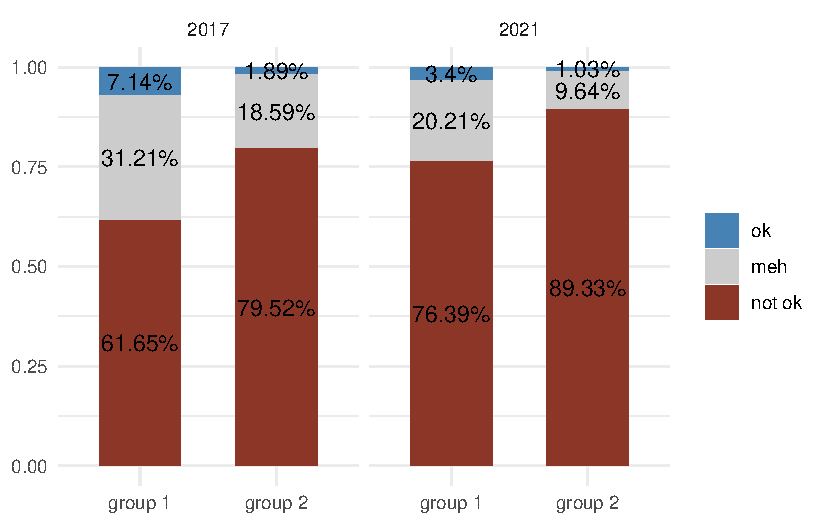
\includegraphics[keepaspectratio]{text_files/figure-pdf/unnamed-chunk-1-1.pdf}}

  We can deal with this using \texttt{geom\_text\_repel()}. Additional
  arguments like \texttt{force} control how much the labels should be
  pushed from their original positions.

\begin{Shaded}
\begin{Highlighting}[]
\FunctionTok{library}\NormalTok{(ggrepel)}

\NormalTok{graph\_df }\SpecialCharTok{\%\textgreater{}\%}
  \FunctionTok{ggplot}\NormalTok{(}\FunctionTok{aes}\NormalTok{(}\AttributeTok{x =}\NormalTok{ target, }\AttributeTok{y =}\NormalTok{ value, }\AttributeTok{fill =}\NormalTok{ att)) }\SpecialCharTok{+}
  \FunctionTok{geom\_col}\NormalTok{(}\AttributeTok{width =}\NormalTok{ .}\DecValTok{6}\NormalTok{) }\SpecialCharTok{+}
  \FunctionTok{geom\_text\_repel}\NormalTok{(}\FunctionTok{aes}\NormalTok{(}\AttributeTok{label =} \FunctionTok{paste0}\NormalTok{(value}\SpecialCharTok{*}\DecValTok{100}\NormalTok{, }\StringTok{"\%"}\NormalTok{)),}\AttributeTok{direction =} \StringTok{"y"}\NormalTok{, }\AttributeTok{position =} \FunctionTok{position\_stack}\NormalTok{(}\AttributeTok{vjust =}\NormalTok{ .}\DecValTok{5}\NormalTok{)) }\SpecialCharTok{+}
  \FunctionTok{scale\_fill\_manual}\NormalTok{(}\AttributeTok{values=} \FunctionTok{c}\NormalTok{(}\StringTok{"ok"}\OtherTok{=} \StringTok{"steelblue"}\NormalTok{,}
                              \StringTok{"meh"} \OtherTok{=} \StringTok{"grey80"}\NormalTok{,}
                              \StringTok{"not ok"} \OtherTok{=} \StringTok{"tomato4"}\NormalTok{)) }\SpecialCharTok{+}
  \FunctionTok{facet\_wrap}\NormalTok{(}\SpecialCharTok{\textasciitilde{}}\NormalTok{year) }\SpecialCharTok{+}
  \FunctionTok{labs}\NormalTok{(}\AttributeTok{x =} \ConstantTok{NULL}\NormalTok{, }\AttributeTok{y =} \ConstantTok{NULL}\NormalTok{) }\SpecialCharTok{+}
  \FunctionTok{theme\_minimal}\NormalTok{() }\SpecialCharTok{+}
  \FunctionTok{theme}\NormalTok{(}\AttributeTok{legend.title =} \FunctionTok{element\_blank}\NormalTok{())}
\end{Highlighting}
\end{Shaded}

  \pandocbounded{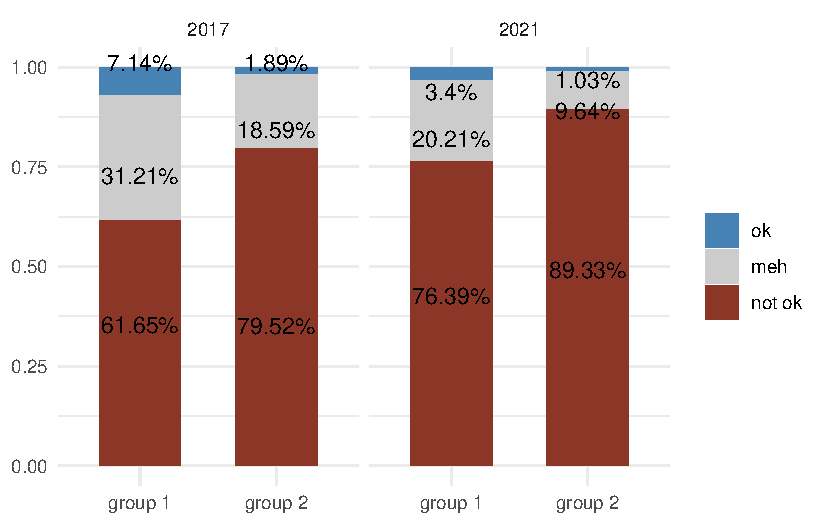
\includegraphics[keepaspectratio]{text_files/figure-pdf/unnamed-chunk-2-1.pdf}}
\item
  ensure proper contrast for text:

  For example the plot below does not have decent contrast when all text
  is in black:

\begin{Shaded}
\begin{Highlighting}[]
\NormalTok{b\_df }\OtherTok{\textless{}{-}} \FunctionTok{data.frame}\NormalTok{(}
    \AttributeTok{a =} \FunctionTok{sample}\NormalTok{(letters[}\DecValTok{1}\SpecialCharTok{:}\DecValTok{5}\NormalTok{], }\FloatTok{1e3}\NormalTok{, }\AttributeTok{replace =}\NormalTok{ T),}
    \AttributeTok{b =} \FunctionTok{sample}\NormalTok{(letters[}\DecValTok{1}\SpecialCharTok{:}\DecValTok{3}\NormalTok{], }\FloatTok{1e3}\NormalTok{, }\AttributeTok{replace =}\NormalTok{ T)}
\NormalTok{) }\SpecialCharTok{\%\textgreater{}\%}
\FunctionTok{count}\NormalTok{(a,b)}

\NormalTok{b\_df }\SpecialCharTok{\%\textgreater{}\%}
\FunctionTok{ggplot}\NormalTok{(}\FunctionTok{aes}\NormalTok{(}\AttributeTok{x =}\NormalTok{ a, }\AttributeTok{y =}\NormalTok{ n, }\AttributeTok{fill =}\NormalTok{ b)) }\SpecialCharTok{+}
\FunctionTok{geom\_col}\NormalTok{(}\AttributeTok{position =} \StringTok{"fill"}\NormalTok{) }\SpecialCharTok{+}
\FunctionTok{geom\_text}\NormalTok{(}\FunctionTok{aes}\NormalTok{(}\AttributeTok{label =}\NormalTok{ n),}\AttributeTok{direction =} \StringTok{"y"}\NormalTok{, }\AttributeTok{position =} \StringTok{"fill"}\NormalTok{, }\AttributeTok{vjust =} \DecValTok{2}\NormalTok{) }\SpecialCharTok{+}
\FunctionTok{scale\_fill\_manual}\NormalTok{(}\AttributeTok{values =} \FunctionTok{c}\NormalTok{(}\StringTok{"grey80"}\NormalTok{, }\StringTok{"firebrick4"}\NormalTok{, }\StringTok{"mistyrose"}\NormalTok{)) }\SpecialCharTok{+}
\FunctionTok{theme\_minimal}\NormalTok{() }\SpecialCharTok{+}
\FunctionTok{theme}\NormalTok{(}\AttributeTok{legend.title =} \FunctionTok{element\_blank}\NormalTok{(),}
     \AttributeTok{legend.position =} \StringTok{"top"}\NormalTok{)}
\end{Highlighting}
\end{Shaded}

\begin{verbatim}
Warning in geom_text(aes(label = n), direction = "y", position = "fill", :
Ignoring unknown parameters: `direction`
\end{verbatim}

  \pandocbounded{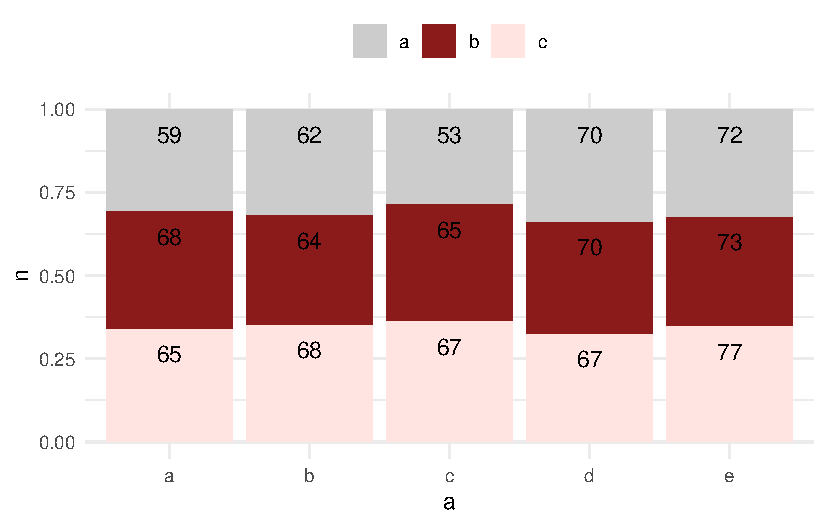
\includegraphics[keepaspectratio]{text_files/figure-pdf/unnamed-chunk-3-1.pdf}}

  We can fix that using \texttt{\{ggfittext\}} and
  \texttt{geom\_fit\_text():}

\begin{Shaded}
\begin{Highlighting}[]
\FunctionTok{library}\NormalTok{(ggfittext)}

\NormalTok{b\_df }\SpecialCharTok{\%\textgreater{}\%}
\FunctionTok{ggplot}\NormalTok{(}\FunctionTok{aes}\NormalTok{(}\AttributeTok{x =}\NormalTok{ a, }\AttributeTok{y =}\NormalTok{ n, }\AttributeTok{fill =}\NormalTok{ b)) }\SpecialCharTok{+}
\FunctionTok{geom\_col}\NormalTok{(}\AttributeTok{position =} \StringTok{"fill"}\NormalTok{) }\SpecialCharTok{+}
\FunctionTok{geom\_fit\_text}\NormalTok{(}\FunctionTok{aes}\NormalTok{(}\AttributeTok{label =}\NormalTok{ n, }\AttributeTok{fill =}\NormalTok{ b), }\AttributeTok{position =} \StringTok{"fill"}\NormalTok{, }\AttributeTok{vjust =} \DecValTok{2}\NormalTok{, }\AttributeTok{contrast =} \ConstantTok{TRUE}\NormalTok{, }\AttributeTok{show\_guide =} \ConstantTok{FALSE}\NormalTok{) }\SpecialCharTok{+}
\FunctionTok{scale\_fill\_manual}\NormalTok{(}\AttributeTok{values =} \FunctionTok{c}\NormalTok{(}\StringTok{"grey80"}\NormalTok{, }\StringTok{"firebrick4"}\NormalTok{, }\StringTok{"mistyrose"}\NormalTok{)) }\SpecialCharTok{+}
\FunctionTok{theme\_minimal}\NormalTok{() }\SpecialCharTok{+}
\FunctionTok{theme}\NormalTok{(}\AttributeTok{legend.title =} \FunctionTok{element\_blank}\NormalTok{(),}
     \AttributeTok{legend.position =} \StringTok{"top"}\NormalTok{)}
\end{Highlighting}
\end{Shaded}

  \pandocbounded{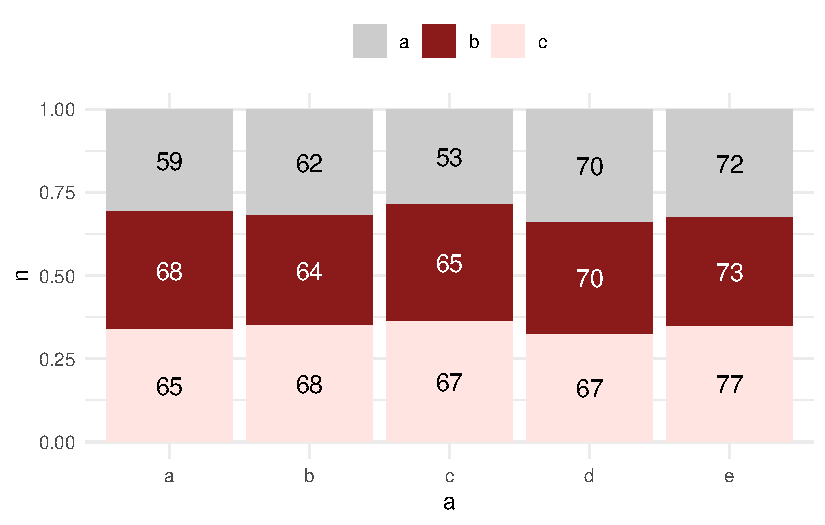
\includegraphics[keepaspectratio]{text_files/figure-pdf/unnamed-chunk-4-1.pdf}}
\item
  Be accessible\ldots{} Don't write about logits. Opt for Average
  Marginal Effects in percentages instead. If possible try to get a
  sense of scale and some interpretation for the effects (maybe
  something like probability of superiority over cohen's d etc.)
\item
  But remain scientific. Be precise, don't overstate - this is
  scientific writing.
\end{itemize}

\bookmarksetup{startatroot}

\chapter{Colors}\label{colors}

This chapter discusses the cbu color palette and preferable ways to use
them

We are working with 2 categorical, 4 continuous (plus grey) and 1
divergent palette.

\section{General rules}\label{general-rules-1}

There are some general rules for working with color

\section{Categorical palette}\label{categorical-palette}

The full categorical palette looks like this:

\begin{Shaded}
\begin{Highlighting}[]
\NormalTok{cbu\_cat }\OtherTok{\textless{}{-}} \FunctionTok{c}\NormalTok{(}\StringTok{"\#b96784"}\NormalTok{, }\StringTok{"\#88375d"}\NormalTok{,}\StringTok{"\#9bb6bd"}\NormalTok{,}\StringTok{"\#5E9FB1"}\NormalTok{, }\StringTok{"\#755687"}\NormalTok{,}\StringTok{"\#4a2d5e"}\NormalTok{, }\StringTok{"\#eb676c"}\NormalTok{,}\StringTok{"\#aa2041"}\NormalTok{, }\StringTok{"\#f2d1ab"}\NormalTok{, }\StringTok{"\#dd9d38"}\NormalTok{)}
\NormalTok{cbu\_cat\_1 }\OtherTok{\textless{}{-}}\NormalTok{ cbu\_cat[}\FunctionTok{c}\NormalTok{(}\DecValTok{1}\SpecialCharTok{:}\DecValTok{5}\NormalTok{)]}
\NormalTok{cbu\_cat\_2 }\OtherTok{\textless{}{-}}\NormalTok{ cbu\_cat[}\FunctionTok{c}\NormalTok{(}\DecValTok{6}\SpecialCharTok{:}\DecValTok{10}\NormalTok{)]}

\FunctionTok{plot\_swatch}\NormalTok{(cbu\_cat, }\AttributeTok{nrow =} \DecValTok{2}\NormalTok{)}
\end{Highlighting}
\end{Shaded}

\pandocbounded{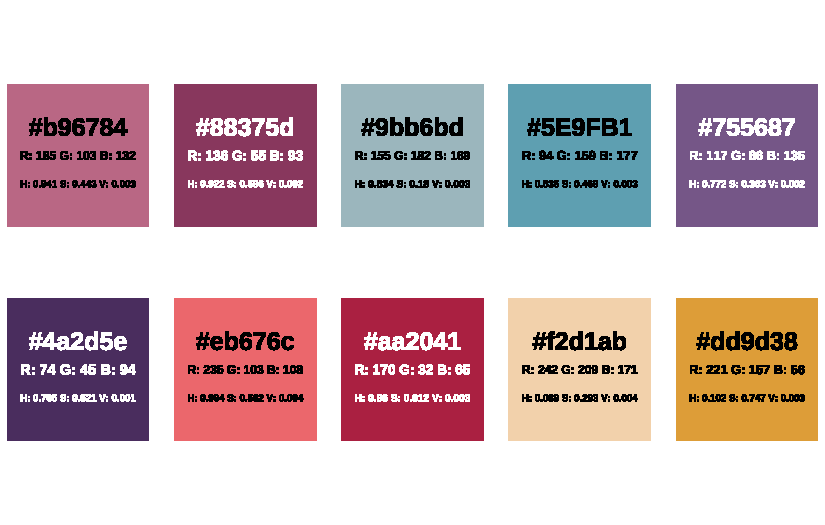
\includegraphics[keepaspectratio]{color_files/figure-pdf/unnamed-chunk-2-1.pdf}}

It can be used in 2 categorical palettes with up to 5 colors each:

\begin{Shaded}
\begin{Highlighting}[]
\FunctionTok{plot\_swatch}\NormalTok{(cbu\_cat\_1)}
\end{Highlighting}
\end{Shaded}

\pandocbounded{\includegraphics[keepaspectratio]{color_files/figure-pdf/unnamed-chunk-3-1.pdf}}

\begin{Shaded}
\begin{Highlighting}[]
\FunctionTok{plot\_swatch}\NormalTok{(cbu\_cat\_2)}
\end{Highlighting}
\end{Shaded}

\pandocbounded{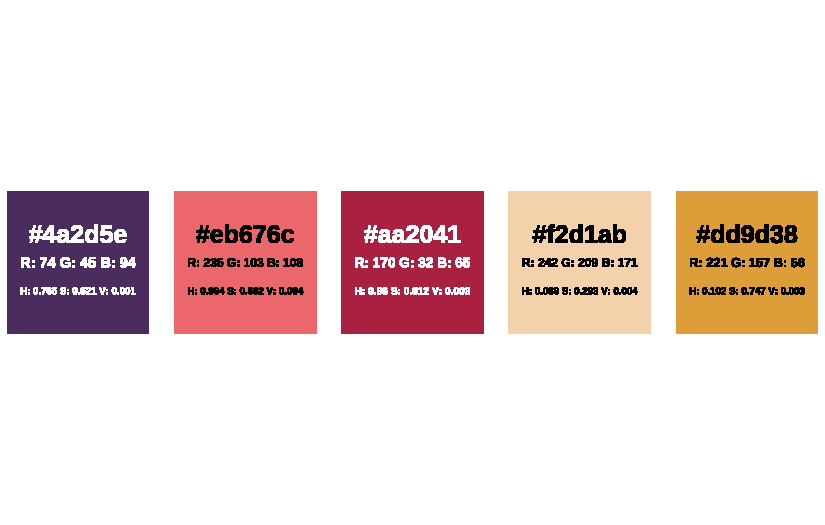
\includegraphics[keepaspectratio]{color_files/figure-pdf/unnamed-chunk-3-2.pdf}}

The categorical palettes should be used in the following order for
increasing number of categories:

\textbf{Palette 1:}

\begin{itemize}
\item
  2 colors: {blush}, and {blue}
\item
  3 colors: {blush}, and {blue}, {purple}
\item
  4 colors: {blush}, and {blue}, {purple} and {magenta}
\end{itemize}

\textbf{Palette 2:}

\begin{itemize}
\item
  2 colors: {light yellow}, and {salmon}
\item
  3 colors: {light yellow}, and {salmon}, {dark purple}
\item
  4 colors: {light yellow}, and {salmon}, {dark purple} and {dark red}
\end{itemize}

Sample plots with those palettes:

\begin{verbatim}
`summarise()` has grouped output by 'marital'. You can override using the
`.groups` argument.
\end{verbatim}

\pandocbounded{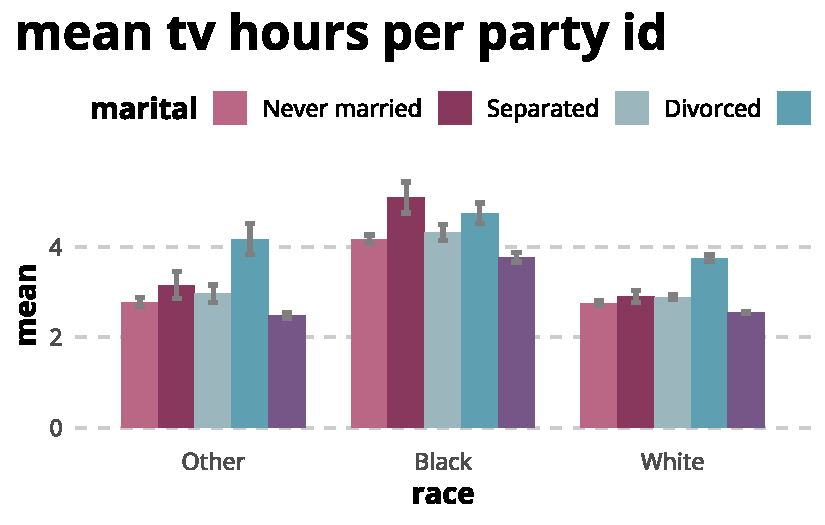
\includegraphics[keepaspectratio]{color_files/figure-pdf/unnamed-chunk-4-1.pdf}}

\begin{verbatim}
`summarise()` has grouped output by 'marital'. You can override using the
`.groups` argument.
\end{verbatim}

\pandocbounded{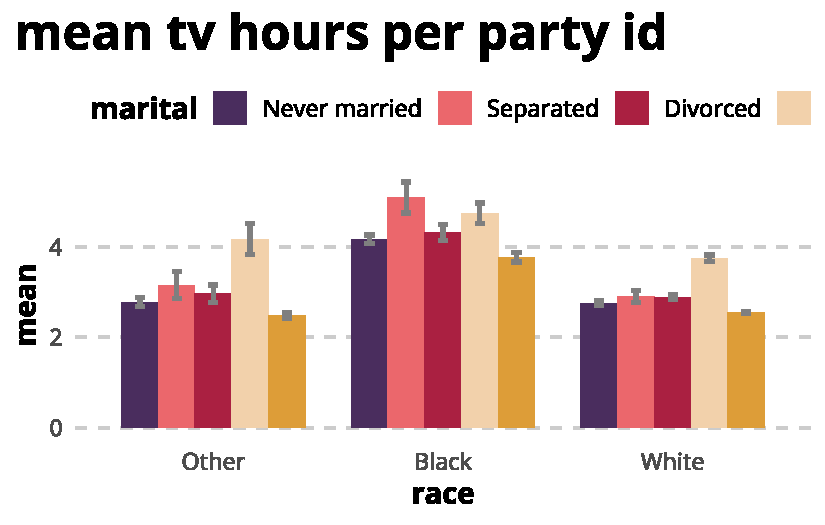
\includegraphics[keepaspectratio]{color_files/figure-pdf/unnamed-chunk-4-2.pdf}}

\section{Continuous palettes}\label{continuous-palettes}

The continuous palettes are bases on the categorical ones with one
palette in greys added.

\begin{Shaded}
\begin{Highlighting}[]
\NormalTok{cbu\_pink }\OtherTok{\textless{}{-}} \FunctionTok{c}\NormalTok{(}\StringTok{\textquotesingle{}\#f79fbc\textquotesingle{}}\NormalTok{, }\StringTok{\textquotesingle{}\#e48dac\textquotesingle{}}\NormalTok{, }\StringTok{\textquotesingle{}\#d17b9b\textquotesingle{}}\NormalTok{, }\StringTok{\textquotesingle{}\#be6a8b\textquotesingle{}}\NormalTok{, }\StringTok{\textquotesingle{}\#ac597b\textquotesingle{}}\NormalTok{, }\StringTok{\textquotesingle{}\#9a486c\textquotesingle{}}\NormalTok{, }\StringTok{\textquotesingle{}\#88375d\textquotesingle{}}\NormalTok{)}

\NormalTok{cbu\_blue }\OtherTok{\textless{}{-}} \FunctionTok{c}\NormalTok{(}\StringTok{\textquotesingle{}\#c4e0e7\textquotesingle{}}\NormalTok{, }\StringTok{\textquotesingle{}\#a6c7d0\textquotesingle{}}\NormalTok{, }\StringTok{\textquotesingle{}\#89afba\textquotesingle{}}\NormalTok{, }\StringTok{\textquotesingle{}\#6c98a4\textquotesingle{}}\NormalTok{, }\StringTok{\textquotesingle{}\#4f818f\textquotesingle{}}\NormalTok{, }\StringTok{\textquotesingle{}\#306b7b\textquotesingle{}}\NormalTok{, }\StringTok{\textquotesingle{}\#005667\textquotesingle{}}\NormalTok{)}

\NormalTok{cbu\_purple }\OtherTok{\textless{}{-}} \FunctionTok{c}\NormalTok{(}\StringTok{\textquotesingle{}\#d0ade3\textquotesingle{}}\NormalTok{, }\StringTok{\textquotesingle{}\#bc9ad0\textquotesingle{}}\NormalTok{, }\StringTok{\textquotesingle{}\#a987bc\textquotesingle{}}\NormalTok{, }\StringTok{\textquotesingle{}\#9675aa\textquotesingle{}}\NormalTok{, }\StringTok{\textquotesingle{}\#836397\textquotesingle{}}\NormalTok{, }\StringTok{\textquotesingle{}\#715285\textquotesingle{}}\NormalTok{, }\StringTok{\textquotesingle{}\#5f4174\textquotesingle{}}\NormalTok{)}

\NormalTok{cbu\_red }\OtherTok{\textless{}{-}} \FunctionTok{c}\NormalTok{(}\StringTok{\textquotesingle{}\#ff9799\textquotesingle{}}\NormalTok{, }\StringTok{\textquotesingle{}\#f18489\textquotesingle{}}\NormalTok{, }\StringTok{\textquotesingle{}\#e3727a\textquotesingle{}}\NormalTok{, }\StringTok{\textquotesingle{}\#d55f6b\textquotesingle{}}\NormalTok{, }\StringTok{\textquotesingle{}\#c74c5d\textquotesingle{}}\NormalTok{, }\StringTok{\textquotesingle{}\#b8384f\textquotesingle{}}\NormalTok{, }\StringTok{\textquotesingle{}\#aa2041\textquotesingle{}}\NormalTok{)}

\NormalTok{cbu\_yellow }\OtherTok{\textless{}{-}} \FunctionTok{c}\NormalTok{(}\StringTok{\textquotesingle{}\#e4b67d\textquotesingle{}}\NormalTok{, }\StringTok{\textquotesingle{}\#d2a368\textquotesingle{}}\NormalTok{, }\StringTok{\textquotesingle{}\#c09054\textquotesingle{}}\NormalTok{, }\StringTok{\textquotesingle{}\#af7e40\textquotesingle{}}\NormalTok{, }\StringTok{\textquotesingle{}\#9d6b2d\textquotesingle{}}\NormalTok{, }\StringTok{\textquotesingle{}\#8b5a18\textquotesingle{}}\NormalTok{, }\StringTok{\textquotesingle{}\#7a4900\textquotesingle{}}\NormalTok{)}
\end{Highlighting}
\end{Shaded}

Sample plots in the continuous palettes are as follows:

\begin{Shaded}
\begin{Highlighting}[]
\NormalTok{cont\_palettes }\OtherTok{\textless{}{-}} \FunctionTok{list}\NormalTok{(cbu\_pink, cbu\_blue, cbu\_purple, cbu\_red, cbu\_yellow)}


\NormalTok{cont\_plot }\OtherTok{\textless{}{-}} \ControlFlowTok{function}\NormalTok{(palette) \{}
\NormalTok{  gss\_cat\_filt }\SpecialCharTok{\%\textgreater{}\%}
  \FunctionTok{group\_by}\NormalTok{(marital) }\SpecialCharTok{\%\textgreater{}\%}
  \FunctionTok{count}\NormalTok{(partyid) }\SpecialCharTok{\%\textgreater{}\%}
  \FunctionTok{mutate}\NormalTok{(}\AttributeTok{perc =} \FunctionTok{round}\NormalTok{(n}\SpecialCharTok{/}\FunctionTok{sum}\NormalTok{(n),}\DecValTok{2}\NormalTok{)) }\SpecialCharTok{\%\textgreater{}\%}
  \FunctionTok{ggplot}\NormalTok{(}\FunctionTok{aes}\NormalTok{(}\AttributeTok{x =}\NormalTok{ marital, }\AttributeTok{y =}\NormalTok{ perc, }\AttributeTok{fill =}\NormalTok{ partyid)) }\SpecialCharTok{+}
  \FunctionTok{geom\_col}\NormalTok{(}\AttributeTok{position =} \StringTok{"fill"}\NormalTok{)}\SpecialCharTok{+}
  \FunctionTok{geom\_text}\NormalTok{(}\FunctionTok{aes}\NormalTok{(}\AttributeTok{label =} \FunctionTok{paste0}\NormalTok{(perc}\SpecialCharTok{*}\DecValTok{100}\NormalTok{, }\StringTok{"\%"}\NormalTok{)), }\AttributeTok{position =} \StringTok{"fill"}\NormalTok{, }\AttributeTok{hjust =} \FloatTok{1.7}\NormalTok{, }\AttributeTok{fontface =} \StringTok{"bold"}\NormalTok{) }\SpecialCharTok{+}
  \FunctionTok{scale\_fill\_manual}\NormalTok{(}\AttributeTok{values=}\NormalTok{ palette) }\SpecialCharTok{+}
  \FunctionTok{labs}\NormalTok{(}\AttributeTok{title =} \StringTok{"Marital status and party id in some gss"}\NormalTok{) }\SpecialCharTok{+}
  \FunctionTok{coord\_flip}\NormalTok{() }\SpecialCharTok{+}
  \FunctionTok{theme\_cbu}\NormalTok{()}
\NormalTok{\}}

\FunctionTok{lapply}\NormalTok{(cont\_palettes, cont\_plot)}
\end{Highlighting}
\end{Shaded}

\begin{verbatim}
[[1]]
\end{verbatim}

\pandocbounded{\includegraphics[keepaspectratio]{color_files/figure-pdf/unnamed-chunk-6-1.pdf}}

\begin{verbatim}

[[2]]
\end{verbatim}

\pandocbounded{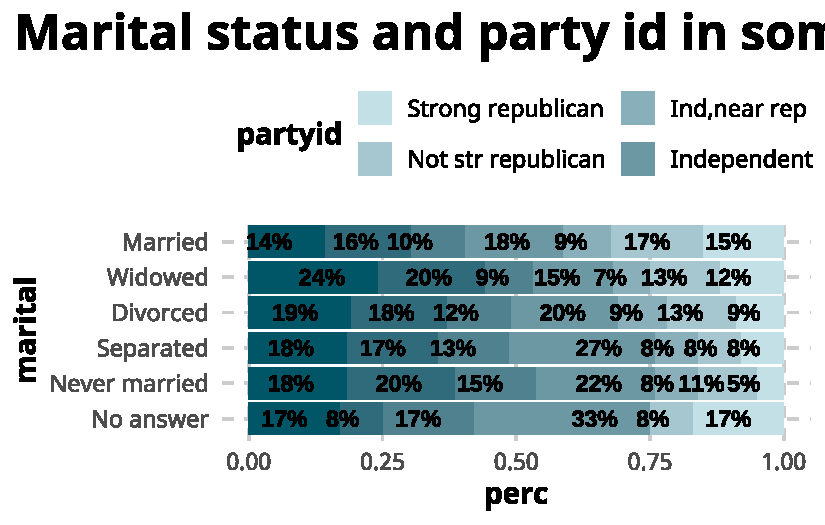
\includegraphics[keepaspectratio]{color_files/figure-pdf/unnamed-chunk-6-2.pdf}}

\begin{verbatim}

[[3]]
\end{verbatim}

\pandocbounded{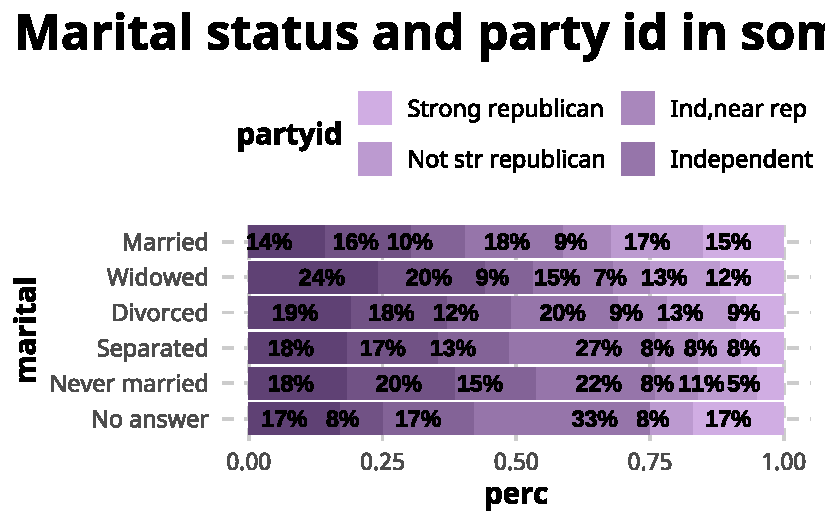
\includegraphics[keepaspectratio]{color_files/figure-pdf/unnamed-chunk-6-3.pdf}}

\begin{verbatim}

[[4]]
\end{verbatim}

\pandocbounded{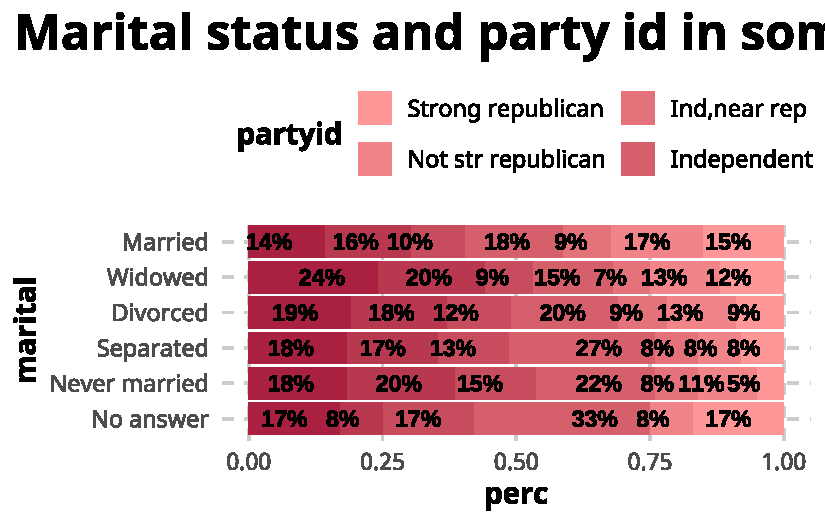
\includegraphics[keepaspectratio]{color_files/figure-pdf/unnamed-chunk-6-4.pdf}}

\begin{verbatim}

[[5]]
\end{verbatim}

\pandocbounded{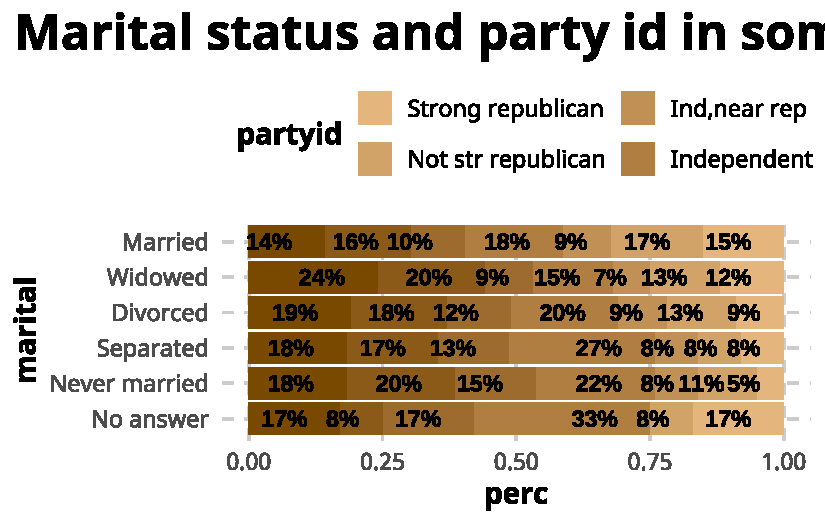
\includegraphics[keepaspectratio]{color_files/figure-pdf/unnamed-chunk-6-5.pdf}}

\section{Divergent palette}\label{divergent-palette}

The divergent palette is created by joining the blue and red continuous
palettes with 1 additional color as the middle point.

\begin{Shaded}
\begin{Highlighting}[]
\NormalTok{cbu\_div }\OtherTok{\textless{}{-}} \FunctionTok{c}\NormalTok{(}\FunctionTok{rev}\NormalTok{(cbu\_blue), }\StringTok{"grey80"}\NormalTok{, cbu\_red)}

\NormalTok{gss\_cat\_filt }\SpecialCharTok{\%\textgreater{}\%}
  \FunctionTok{ggplot}\NormalTok{(}\FunctionTok{aes}\NormalTok{(}\AttributeTok{x =}\NormalTok{ marital, }\AttributeTok{fill =} \FunctionTok{factor}\NormalTok{(partyid))) }\SpecialCharTok{+}
  \FunctionTok{geom\_bar}\NormalTok{(}\AttributeTok{position =} \StringTok{"fill"}\NormalTok{)}\SpecialCharTok{+}
  \FunctionTok{scale\_fill\_manual}\NormalTok{(}\AttributeTok{values=}\NormalTok{ cbu\_div[}\FunctionTok{c}\NormalTok{(}\DecValTok{2}\NormalTok{,}\DecValTok{4}\NormalTok{,}\DecValTok{6}\NormalTok{,}\DecValTok{8}\NormalTok{,}\DecValTok{11}\NormalTok{,}\DecValTok{13}\NormalTok{,}\DecValTok{15}\NormalTok{)]) }\SpecialCharTok{+}
  \FunctionTok{labs}\NormalTok{(}\AttributeTok{title =} \StringTok{"Marital status and party id in some gss"}\NormalTok{) }\SpecialCharTok{+}
  \FunctionTok{coord\_flip}\NormalTok{() }\SpecialCharTok{+}
  \FunctionTok{theme\_cbu}\NormalTok{()}
\end{Highlighting}
\end{Shaded}

\pandocbounded{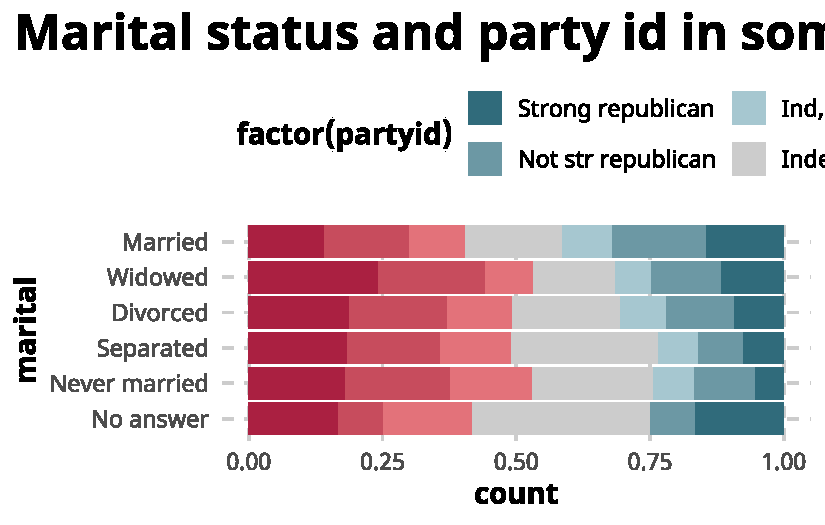
\includegraphics[keepaspectratio]{color_files/figure-pdf/unnamed-chunk-7-1.pdf}}

\bookmarksetup{startatroot}

\chapter{Theme}\label{theme}

This chapter discusses the \texttt{cbu\_theme()} function for styling
the ggplot objects into cbu-styled plots.

\textbf{note}: should we have logo on the plots?

\section{The function}\label{the-function}

Put the function here and discuss it a bit.

\begin{Shaded}
\begin{Highlighting}[]
\FunctionTok{library}\NormalTok{(tidyverse)}
\FunctionTok{library}\NormalTok{(showtext)}

\FunctionTok{font\_add\_google}\NormalTok{(}\StringTok{"Open Sans"}\NormalTok{)}
\FunctionTok{showtext\_auto}\NormalTok{()}
\NormalTok{font }\OtherTok{\textless{}{-}} \StringTok{"Open Sans"}


\NormalTok{cbu\_cat }\OtherTok{\textless{}{-}} \FunctionTok{c}\NormalTok{(}\StringTok{"\#b96784"}\NormalTok{, }\StringTok{"\#88375d"}\NormalTok{,}\StringTok{"\#9bb6bd"}\NormalTok{,}\StringTok{"\#5E9FB1"}\NormalTok{, }\StringTok{"\#755687"}\NormalTok{,}\StringTok{"\#4a2d5e"}\NormalTok{, }\StringTok{"\#eb676c"}\NormalTok{,}\StringTok{"\#aa2041"}\NormalTok{, }\StringTok{"\#f2d1ab"}\NormalTok{, }\StringTok{"\#dd9d38"}\NormalTok{)}
\NormalTok{cbu\_cat\_1 }\OtherTok{\textless{}{-}}\NormalTok{ cbu\_cat[}\FunctionTok{c}\NormalTok{(}\DecValTok{1}\SpecialCharTok{:}\DecValTok{5}\NormalTok{)]}
\NormalTok{cbu\_cat\_2 }\OtherTok{\textless{}{-}}\NormalTok{ cbu\_cat[}\FunctionTok{c}\NormalTok{(}\DecValTok{6}\SpecialCharTok{:}\DecValTok{10}\NormalTok{)]}

\NormalTok{theme\_cbu }\OtherTok{\textless{}{-}} \ControlFlowTok{function}\NormalTok{() \{}
  \FunctionTok{theme\_minimal}\NormalTok{(}\AttributeTok{base\_size =} \DecValTok{14}\NormalTok{, }\AttributeTok{base\_family =}\NormalTok{ font) }\SpecialCharTok{+}
    \FunctionTok{theme}\NormalTok{(}\AttributeTok{panel.grid.minor =} \FunctionTok{element\_blank}\NormalTok{(),}
          \AttributeTok{panel.grid.major =} \FunctionTok{element\_line}\NormalTok{(}\AttributeTok{color =} \StringTok{"grey80"}\NormalTok{, }\AttributeTok{linewidth =}\NormalTok{ .}\DecValTok{5}\NormalTok{),}
          \AttributeTok{panel.grid.major.x =} \FunctionTok{element\_blank}\NormalTok{(),}
          \AttributeTok{plot.background =} \FunctionTok{element\_rect}\NormalTok{(}\AttributeTok{fill =} \StringTok{"white"}\NormalTok{, }\AttributeTok{color =} \ConstantTok{NA}\NormalTok{),}
          \AttributeTok{plot.title =} \FunctionTok{element\_text}\NormalTok{(}\AttributeTok{size =} \FloatTok{1.68}\SpecialCharTok{*}\DecValTok{12}\NormalTok{, }\AttributeTok{face =} \StringTok{"bold"}\NormalTok{, }\AttributeTok{family =}\NormalTok{ font),}
          \AttributeTok{plot.subtitle =} \FunctionTok{element\_text}\NormalTok{(}\AttributeTok{face =} \StringTok{"italic"}\NormalTok{, }\AttributeTok{family =}\NormalTok{ font),}
          \AttributeTok{axis.title =} \FunctionTok{element\_text}\NormalTok{(}\AttributeTok{face =} \StringTok{"bold"}\NormalTok{, }\AttributeTok{size =} \FloatTok{8.5}\NormalTok{),}
          \AttributeTok{axis.text =} \FunctionTok{element\_text}\NormalTok{(}\AttributeTok{size =} \DecValTok{8}\NormalTok{),}
          \AttributeTok{strip.text =} \FunctionTok{element\_text}\NormalTok{(}\AttributeTok{face =} \StringTok{"bold"}\NormalTok{, }\AttributeTok{size =} \DecValTok{10}\NormalTok{),}
          \AttributeTok{strip.background =} \FunctionTok{element\_rect}\NormalTok{(}\AttributeTok{fill =} \ConstantTok{NA}\NormalTok{, }\AttributeTok{color =} \ConstantTok{NA}\NormalTok{),}
          \AttributeTok{plot.caption =} \FunctionTok{element\_text}\NormalTok{(}\AttributeTok{face =} \StringTok{"italic"}\NormalTok{, }\AttributeTok{family =}\NormalTok{ font, }\AttributeTok{size =} \DecValTok{8}\NormalTok{),}
          \AttributeTok{legend.title =} \FunctionTok{element\_text}\NormalTok{(}\AttributeTok{face =} \StringTok{"bold"}\NormalTok{, }\AttributeTok{size =} \DecValTok{10}\NormalTok{),}
          \AttributeTok{legend.text =} \FunctionTok{element\_text}\NormalTok{(}\AttributeTok{size =} \DecValTok{10}\NormalTok{),}
          \AttributeTok{legend.key.size =} \FunctionTok{unit}\NormalTok{(}\DecValTok{10}\NormalTok{, }\StringTok{"pt"}\NormalTok{),}
          \AttributeTok{legend.position =} \StringTok{"top"}\NormalTok{,}
          \AttributeTok{legend.justification=}\StringTok{\textquotesingle{}left\textquotesingle{}}\NormalTok{,}
          \AttributeTok{legend.direction=}\StringTok{\textquotesingle{}horizontal\textquotesingle{}}\NormalTok{,}
          \AttributeTok{plot.margin =} \FunctionTok{unit}\NormalTok{(}\FunctionTok{c}\NormalTok{(}\AttributeTok{t =}\DecValTok{0}\NormalTok{, }\AttributeTok{r =} \DecValTok{0}\NormalTok{, }\AttributeTok{b =} \DecValTok{0}\NormalTok{, }\AttributeTok{l =} \DecValTok{0}\NormalTok{), }\StringTok{"cm"}\NormalTok{)}
\NormalTok{          )}
\NormalTok{\}}
\end{Highlighting}
\end{Shaded}

The function is based on theme minimal. It uses \textbf{Open Sans font}
with base size of \textbf{14}. The main idea behind the theme function
was to declutter the plot and take care of some basic layout \& text
hierarchy (especially the legend which can be rendered a bit awkwardly
by default).

\section{How it looks like}\label{how-it-looks-like}

Here is a sample plot:

\begin{Shaded}
\begin{Highlighting}[]
\NormalTok{some\_df }\OtherTok{\textless{}{-}} \FunctionTok{data.frame}\NormalTok{(}
    \AttributeTok{a =} \FunctionTok{sample}\NormalTok{(letters[}\DecValTok{1}\SpecialCharTok{:}\DecValTok{7}\NormalTok{], }\DecValTok{1000}\NormalTok{, }\AttributeTok{replace =}\NormalTok{ T)}
\NormalTok{) }\SpecialCharTok{\%\textgreater{}\%}
\FunctionTok{count}\NormalTok{(a)}

\NormalTok{some\_df }\SpecialCharTok{\%\textgreater{}\%}
\FunctionTok{ggplot}\NormalTok{(}\FunctionTok{aes}\NormalTok{(}\AttributeTok{x =}\NormalTok{ a, }\AttributeTok{y =}\NormalTok{ n)) }\SpecialCharTok{+}
\FunctionTok{geom\_col}\NormalTok{(}\AttributeTok{fill =}\NormalTok{ cbu\_cat\_1[}\DecValTok{1}\NormalTok{], }\AttributeTok{width =}\NormalTok{ .}\DecValTok{6}\NormalTok{) }\SpecialCharTok{+}
\FunctionTok{geom\_text}\NormalTok{(}\FunctionTok{aes}\NormalTok{(}\AttributeTok{label =}\NormalTok{ n), }\AttributeTok{nudge\_y =} \DecValTok{2}\NormalTok{, }\AttributeTok{size =} \DecValTok{3}\NormalTok{) }\SpecialCharTok{+}
\FunctionTok{labs}\NormalTok{(}\AttributeTok{x =} \StringTok{"letters"}\NormalTok{, }\AttributeTok{y =} \StringTok{"counts"}\NormalTok{) }\SpecialCharTok{+}
\FunctionTok{coord\_flip}\NormalTok{() }\SpecialCharTok{+}
\FunctionTok{theme\_cbu}\NormalTok{()}
\end{Highlighting}
\end{Shaded}

\pandocbounded{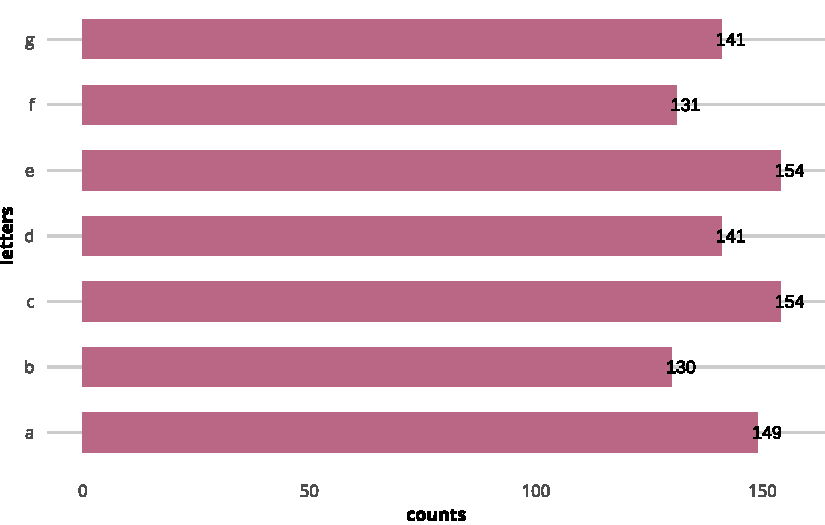
\includegraphics[keepaspectratio]{theme_files/figure-pdf/unnamed-chunk-2-1.pdf}}

Another example with continuous variables:

\begin{Shaded}
\begin{Highlighting}[]
\NormalTok{cont\_df }\OtherTok{\textless{}{-}} \FunctionTok{data.frame}\NormalTok{(}\AttributeTok{x =} \FunctionTok{runif}\NormalTok{(}\FloatTok{1e3}\NormalTok{, }\DecValTok{0}\NormalTok{, }\DecValTok{4}\NormalTok{),}
                      \AttributeTok{a =} \FunctionTok{sample}\NormalTok{(letters[}\DecValTok{1}\SpecialCharTok{:}\DecValTok{3}\NormalTok{], }\FloatTok{1e3}\NormalTok{, }\AttributeTok{replace =}\NormalTok{ T)) }\SpecialCharTok{\%\textgreater{}\%}
  \FunctionTok{mutate}\NormalTok{(}\AttributeTok{y =} \FunctionTok{ifelse}\NormalTok{(a }\SpecialCharTok{==} \StringTok{"a"}\NormalTok{,}
                    \FunctionTok{rnorm}\NormalTok{(}\FloatTok{1e3}\NormalTok{, }\AttributeTok{mean =} \FunctionTok{sin}\NormalTok{(x) }\SpecialCharTok{+} \DecValTok{3}\SpecialCharTok{*}\FunctionTok{cos}\NormalTok{(x}\SpecialCharTok{\^{}}\DecValTok{2}\NormalTok{) }\SpecialCharTok{{-}}\NormalTok{ x}\SpecialCharTok{\^{}}\DecValTok{2} \SpecialCharTok{+}\NormalTok{ .}\DecValTok{5}\SpecialCharTok{*}\NormalTok{x}\SpecialCharTok{\^{}}\DecValTok{3}\NormalTok{),}
                    \FunctionTok{ifelse}\NormalTok{(a }\SpecialCharTok{==} \StringTok{"b"}\NormalTok{,}
                           \FunctionTok{rnorm}\NormalTok{(}\FloatTok{1e3}\NormalTok{, }\AttributeTok{mean =} \SpecialCharTok{{-}}\FunctionTok{sin}\NormalTok{(x) }\SpecialCharTok{+} \DecValTok{3}\SpecialCharTok{*}\FunctionTok{cos}\NormalTok{(x}\SpecialCharTok{\^{}}\DecValTok{2}\NormalTok{) }\SpecialCharTok{+}\NormalTok{ x}\SpecialCharTok{\^{}}\DecValTok{2} \SpecialCharTok{{-}}\NormalTok{ .}\DecValTok{2}\SpecialCharTok{*}\NormalTok{x}\SpecialCharTok{\^{}}\DecValTok{3}\NormalTok{),}
                           \FunctionTok{rnorm}\NormalTok{(}\FloatTok{1e3}\NormalTok{, }\AttributeTok{mean =} \DecValTok{6} \SpecialCharTok{+} \DecValTok{2}\SpecialCharTok{*}\FunctionTok{sin}\NormalTok{(x) }\SpecialCharTok{{-}} \FloatTok{1.5}\SpecialCharTok{*}\FunctionTok{cos}\NormalTok{(x}\SpecialCharTok{\^{}}\DecValTok{2}\NormalTok{) }\SpecialCharTok{{-}}\NormalTok{ x}\SpecialCharTok{\^{}}\DecValTok{2} \SpecialCharTok{+}\NormalTok{ .}\DecValTok{5}\SpecialCharTok{*}\NormalTok{x}\SpecialCharTok{\^{}}\DecValTok{3}\NormalTok{))))}
           


\NormalTok{cont\_df }\SpecialCharTok{\%\textgreater{}\%}
  \FunctionTok{ggplot}\NormalTok{(}\FunctionTok{aes}\NormalTok{(}\AttributeTok{x =}\NormalTok{ x, }\AttributeTok{y =}\NormalTok{ y, }\AttributeTok{color =}\NormalTok{ a)) }\SpecialCharTok{+}
  \FunctionTok{geom\_point}\NormalTok{(}\AttributeTok{alpha =}\NormalTok{ .}\DecValTok{5}\NormalTok{) }\SpecialCharTok{+}
  \FunctionTok{geom\_smooth}\NormalTok{(}\AttributeTok{method =} \StringTok{"gam"}\NormalTok{, }\AttributeTok{se =}\NormalTok{ F) }\SpecialCharTok{+}
  \FunctionTok{scale\_color\_manual}\NormalTok{(}\AttributeTok{values =}\NormalTok{ cbu\_cat\_2[}\FunctionTok{c}\NormalTok{(}\DecValTok{2}\NormalTok{,}\DecValTok{4}\NormalTok{,}\DecValTok{1}\NormalTok{)]) }\SpecialCharTok{+}
  \FunctionTok{labs}\NormalTok{(}\AttributeTok{x =} \StringTok{"jakiś czas"}\NormalTok{, }\AttributeTok{y =} \StringTok{"jakaś ilościowa"}\NormalTok{, }\AttributeTok{color =} \StringTok{"category"}\NormalTok{) }\SpecialCharTok{+}
  \FunctionTok{theme\_cbu}\NormalTok{()}
\end{Highlighting}
\end{Shaded}

\begin{verbatim}
`geom_smooth()` using formula = 'y ~ s(x, bs = "cs")'
\end{verbatim}

\pandocbounded{\includegraphics[keepaspectratio]{theme_files/figure-pdf/unnamed-chunk-3-1.pdf}}

Below is a breakdown of all elements in the theme:

\pandocbounded{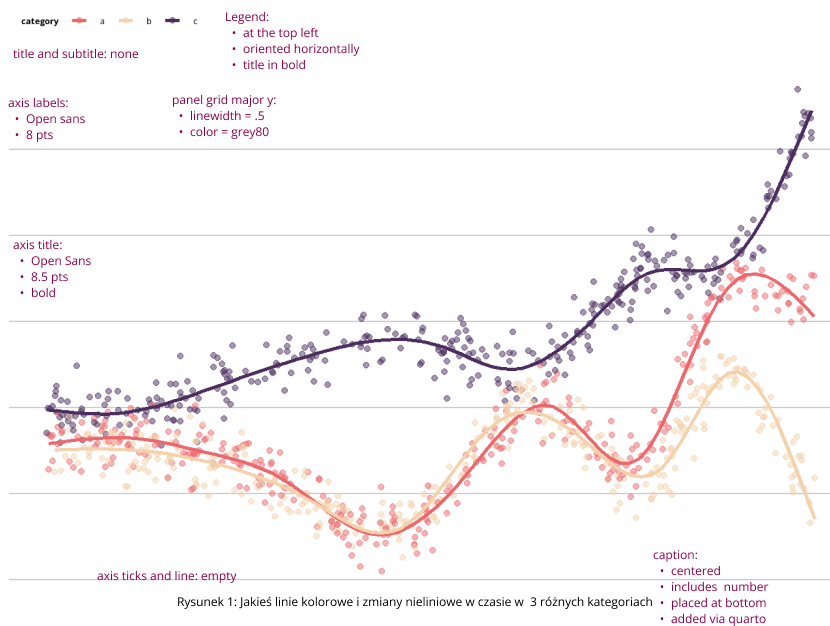
\includegraphics[keepaspectratio]{images/clipboard-1620097183.png}}

\section{Table theming}\label{table-theming}

Cbu report format works on typst which necessitates using
\texttt{\{tinytable\}} package for making table as it is currently the
only one that supports rendering in typst without problems. The main 2
types of tables used in cbu reports are ones containing primarily
numbers (e.g.~summary statistics, reporting model coefficients) and ones
containing primarily text (e.g.~item wording). Those can be styled a bit
differently to fit conventions and the particular content.

\subsection{Tables with numbers}\label{tables-with-numbers}

These tables include things like tables with sample characteristics
(e.g.~age, gender, education, place of living etc), summary statistics
like means and standard deviations for important variables etc.

\subsection{Text tables}\label{text-tables}

These tables include tables that primarily present text, especially when
presenting scale items.

issues:

\begin{itemize}
\item
  long text
\item
  merging cells
\end{itemize}

\subsection{Model output tables}\label{model-output-tables}

These tables include any statistical models presented in table format.

\begin{itemize}
\item
  which information should be included
\item
  text tables:

  \begin{itemize}
  \item
    issues: long text
  \item
    merging cells
  \end{itemize}
\item
  model output tables:

  \begin{itemize}
  \tightlist
  \item
    general information that should be included in a table that
    describes a model are pretty much the same as standard APA stuff:
    include uncertainty (standard errors or confidence intervals)
  \end{itemize}
\end{itemize}

\bookmarksetup{startatroot}

\chapter{Chart types}\label{chart-types}

This part discusses specific types of charts, when to use them and some
tweaks to make them work.

Center for Research on Prejudice reports can contain various types of
plots but there are some common ones that appear more often then others
and also have some specific issues related to them. This section
provides some suggestions on how to build specific types of charts and
how to address the issues that arise with each of those types.

\begin{Shaded}
\begin{Highlighting}[]
\FunctionTok{library}\NormalTok{(tidyverse)}
\end{Highlighting}
\end{Shaded}

\begin{verbatim}
-- Attaching core tidyverse packages ------------------------ tidyverse 2.0.0 --
v dplyr     1.1.4     v readr     2.1.5
v forcats   1.0.0     v stringr   1.5.1
v ggplot2   3.5.1     v tibble    3.2.1
v lubridate 1.9.4     v tidyr     1.3.1
v purrr     1.0.4     
-- Conflicts ------------------------------------------ tidyverse_conflicts() --
x dplyr::filter() masks stats::filter()
x dplyr::lag()    masks stats::lag()
i Use the conflicted package (<http://conflicted.r-lib.org/>) to force all conflicts to become errors
\end{verbatim}

\begin{Shaded}
\begin{Highlighting}[]
\FunctionTok{library}\NormalTok{(showtext)}
\end{Highlighting}
\end{Shaded}

\begin{verbatim}
Loading required package: sysfonts
Loading required package: showtextdb
\end{verbatim}

\begin{Shaded}
\begin{Highlighting}[]
\FunctionTok{library}\NormalTok{(ggrepel)}
\FunctionTok{library}\NormalTok{(ggfittext)}
\FunctionTok{font\_add\_google}\NormalTok{(}\StringTok{"Open Sans"}\NormalTok{)}
\FunctionTok{showtext\_auto}\NormalTok{()}
\NormalTok{font }\OtherTok{\textless{}{-}} \StringTok{"Open Sans"}


\NormalTok{cbu\_cat }\OtherTok{\textless{}{-}} \FunctionTok{c}\NormalTok{(}\StringTok{"\#b96784"}\NormalTok{, }\StringTok{"\#88375d"}\NormalTok{,}\StringTok{"\#9bb6bd"}\NormalTok{,}\StringTok{"\#5E9FB1"}\NormalTok{, }\StringTok{"\#755687"}\NormalTok{,}\StringTok{"\#4a2d5e"}\NormalTok{, }\StringTok{"\#eb676c"}\NormalTok{,}\StringTok{"\#aa2041"}\NormalTok{, }\StringTok{"\#f2d1ab"}\NormalTok{, }\StringTok{"\#dd9d38"}\NormalTok{)}
\NormalTok{cbu\_cat\_1 }\OtherTok{\textless{}{-}}\NormalTok{ cbu\_cat[}\FunctionTok{c}\NormalTok{(}\DecValTok{1}\SpecialCharTok{:}\DecValTok{5}\NormalTok{)]}
\NormalTok{cbu\_cat\_2 }\OtherTok{\textless{}{-}}\NormalTok{ cbu\_cat[}\FunctionTok{c}\NormalTok{(}\DecValTok{6}\SpecialCharTok{:}\DecValTok{10}\NormalTok{)]}

\NormalTok{theme\_cbu }\OtherTok{\textless{}{-}} \ControlFlowTok{function}\NormalTok{() \{}
  \FunctionTok{theme\_minimal}\NormalTok{(}\AttributeTok{base\_size =} \DecValTok{14}\NormalTok{, }\AttributeTok{base\_family =}\NormalTok{ font) }\SpecialCharTok{+}
    \FunctionTok{theme}\NormalTok{(}\AttributeTok{panel.grid.minor =} \FunctionTok{element\_blank}\NormalTok{(),}
          \AttributeTok{panel.grid.major =} \FunctionTok{element\_line}\NormalTok{(}\AttributeTok{color =} \StringTok{"grey80"}\NormalTok{, }\AttributeTok{linewidth =}\NormalTok{ .}\DecValTok{5}\NormalTok{),}
          \AttributeTok{panel.grid.major.x =} \FunctionTok{element\_blank}\NormalTok{(),}
          \AttributeTok{plot.background =} \FunctionTok{element\_rect}\NormalTok{(}\AttributeTok{fill =} \StringTok{"white"}\NormalTok{, }\AttributeTok{color =} \ConstantTok{NA}\NormalTok{),}
          \AttributeTok{plot.title =} \FunctionTok{element\_text}\NormalTok{(}\AttributeTok{size =} \FloatTok{1.68}\SpecialCharTok{*}\DecValTok{12}\NormalTok{, }\AttributeTok{face =} \StringTok{"bold"}\NormalTok{, }\AttributeTok{family =}\NormalTok{ font),}
          \AttributeTok{plot.subtitle =} \FunctionTok{element\_text}\NormalTok{(}\AttributeTok{face =} \StringTok{"italic"}\NormalTok{, }\AttributeTok{family =}\NormalTok{ font),}
          \AttributeTok{axis.title =} \FunctionTok{element\_text}\NormalTok{(}\AttributeTok{face =} \StringTok{"bold"}\NormalTok{, }\AttributeTok{size =} \FloatTok{8.5}\NormalTok{),}
          \AttributeTok{axis.text =} \FunctionTok{element\_text}\NormalTok{(}\AttributeTok{size =} \DecValTok{8}\NormalTok{),}
          \AttributeTok{strip.text =} \FunctionTok{element\_text}\NormalTok{(}\AttributeTok{face =} \StringTok{"bold"}\NormalTok{, }\AttributeTok{size =} \DecValTok{10}\NormalTok{),}
          \AttributeTok{strip.background =} \FunctionTok{element\_rect}\NormalTok{(}\AttributeTok{fill =} \ConstantTok{NA}\NormalTok{, }\AttributeTok{color =} \ConstantTok{NA}\NormalTok{),}
          \AttributeTok{plot.caption =} \FunctionTok{element\_text}\NormalTok{(}\AttributeTok{face =} \StringTok{"italic"}\NormalTok{, }\AttributeTok{family =}\NormalTok{ font, }\AttributeTok{size =} \DecValTok{8}\NormalTok{),}
          \AttributeTok{legend.title =} \FunctionTok{element\_text}\NormalTok{(}\AttributeTok{face =} \StringTok{"bold"}\NormalTok{, }\AttributeTok{size =} \DecValTok{10}\NormalTok{),}
          \AttributeTok{legend.text =} \FunctionTok{element\_text}\NormalTok{(}\AttributeTok{size =} \DecValTok{10}\NormalTok{),}
          \AttributeTok{legend.key.size =} \FunctionTok{unit}\NormalTok{(}\DecValTok{10}\NormalTok{, }\StringTok{"pt"}\NormalTok{),}
          \AttributeTok{legend.position =} \StringTok{"top"}\NormalTok{,}
          \AttributeTok{legend.justification=}\StringTok{\textquotesingle{}left\textquotesingle{}}\NormalTok{,}
          \AttributeTok{legend.direction=}\StringTok{\textquotesingle{}horizontal\textquotesingle{}}\NormalTok{,}
          \AttributeTok{plot.margin =} \FunctionTok{unit}\NormalTok{(}\FunctionTok{c}\NormalTok{(}\AttributeTok{t =}\DecValTok{0}\NormalTok{, }\AttributeTok{r =} \DecValTok{0}\NormalTok{, }\AttributeTok{b =} \DecValTok{0}\NormalTok{, }\AttributeTok{l =} \DecValTok{0}\NormalTok{), }\StringTok{"cm"}\NormalTok{)}
\NormalTok{          )}
\NormalTok{\}}
\end{Highlighting}
\end{Shaded}

\subsection{Bar charts}\label{bar-charts}

We'll start with bar charts. Those are pretty common in cbu reports for
showing and comparing means or counts. Some general rules to follow here
are:

\begin{itemize}
\item
  if possible add text above the bars
\item
  make the bars a bit thinner than default ggplot behaviour
\item
  Unless necessary don't use multiple colors
\end{itemize}

Here is an example of a cbu styled bar plot showing some means:

\begin{Shaded}
\begin{Highlighting}[]
\NormalTok{bar\_df }\OtherTok{\textless{}{-}} \FunctionTok{data.frame}\NormalTok{(}
    \AttributeTok{category =}\NormalTok{ letters[}\DecValTok{1}\SpecialCharTok{:}\DecValTok{7}\NormalTok{],}
    \AttributeTok{means =} \FunctionTok{round}\NormalTok{(}\FunctionTok{rnorm}\NormalTok{(}\DecValTok{7}\NormalTok{, }\DecValTok{6}\NormalTok{, }\FloatTok{1.5}\NormalTok{), }\DecValTok{2}\NormalTok{)}
\NormalTok{)}

\NormalTok{bar\_df }\SpecialCharTok{\%\textgreater{}\%}
\FunctionTok{ggplot}\NormalTok{(}\FunctionTok{aes}\NormalTok{(}\AttributeTok{x =}\NormalTok{ category, }\AttributeTok{y =}\NormalTok{ means)) }\SpecialCharTok{+}
\FunctionTok{geom\_col}\NormalTok{(}\AttributeTok{fill=}\NormalTok{ cbu\_cat\_1[}\DecValTok{1}\NormalTok{], }\AttributeTok{width =}\NormalTok{ .}\DecValTok{6}\NormalTok{) }\SpecialCharTok{+}
\FunctionTok{geom\_text}\NormalTok{(}\FunctionTok{aes}\NormalTok{(}\AttributeTok{label =}\NormalTok{ means), }\AttributeTok{nudge\_y =}\NormalTok{ .}\DecValTok{5}\NormalTok{) }\SpecialCharTok{+}
\FunctionTok{theme\_cbu}\NormalTok{()}
\end{Highlighting}
\end{Shaded}

\pandocbounded{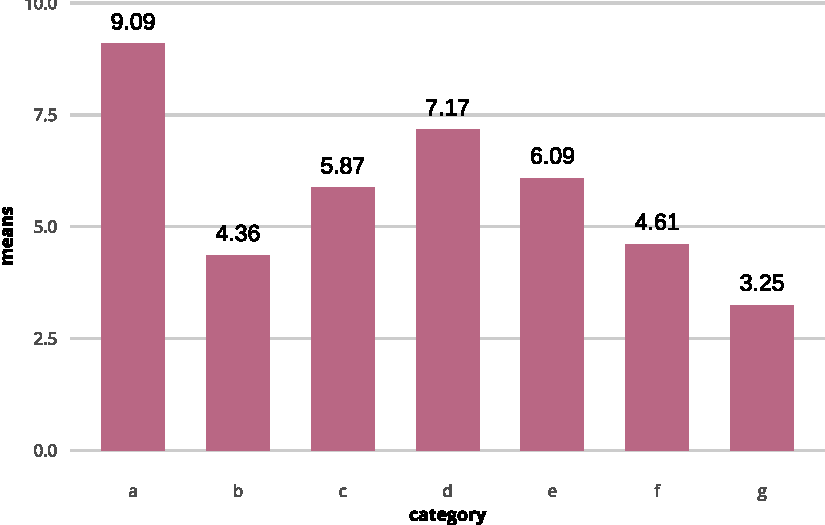
\includegraphics[keepaspectratio]{chart_types_files/figure-pdf/unnamed-chunk-2-1.pdf}}

A few more specific issues that often arise for bar plots:

\begin{itemize}
\item
  position adjustments\\
  Bar plot work best with position dodge. The only thing to remember is
  to set the width right and add the position adjustment to any
  additional geoms used in the plot.

\begin{Shaded}
\begin{Highlighting}[]
\NormalTok{bar\_df}\SpecialCharTok{$}\NormalTok{category\_2 }\OtherTok{\textless{}{-}} \FunctionTok{c}\NormalTok{(}\FunctionTok{rep}\NormalTok{(}\StringTok{"a"}\NormalTok{, }\DecValTok{3}\NormalTok{), }\FunctionTok{rep}\NormalTok{(}\StringTok{"b"}\NormalTok{, }\DecValTok{4}\NormalTok{))}

\NormalTok{bar\_df }\SpecialCharTok{\%\textgreater{}\%}
\FunctionTok{ggplot}\NormalTok{(}\FunctionTok{aes}\NormalTok{(}\AttributeTok{x =}\NormalTok{ category\_2, }\AttributeTok{y =}\NormalTok{ means, }\AttributeTok{fill =}\NormalTok{ category)) }\SpecialCharTok{+}
\FunctionTok{geom\_col}\NormalTok{(}\AttributeTok{width =}\NormalTok{ .}\DecValTok{6}\NormalTok{, }\AttributeTok{position =} \FunctionTok{position\_dodge}\NormalTok{(}\AttributeTok{width =}\NormalTok{ .}\DecValTok{6}\NormalTok{)) }\SpecialCharTok{+}
\FunctionTok{geom\_text}\NormalTok{(}\FunctionTok{aes}\NormalTok{(}\AttributeTok{label =}\NormalTok{ means),}\AttributeTok{position =} \FunctionTok{position\_dodge}\NormalTok{(}\AttributeTok{width =}\NormalTok{ .}\DecValTok{6}\NormalTok{), }\AttributeTok{vjust =} \DecValTok{1}\NormalTok{) }\SpecialCharTok{+}
\FunctionTok{scale\_fill\_manual}\NormalTok{(}\AttributeTok{values =}\NormalTok{ cbu\_cat) }\SpecialCharTok{+}
\FunctionTok{theme\_cbu}\NormalTok{()}
\end{Highlighting}
\end{Shaded}

  \pandocbounded{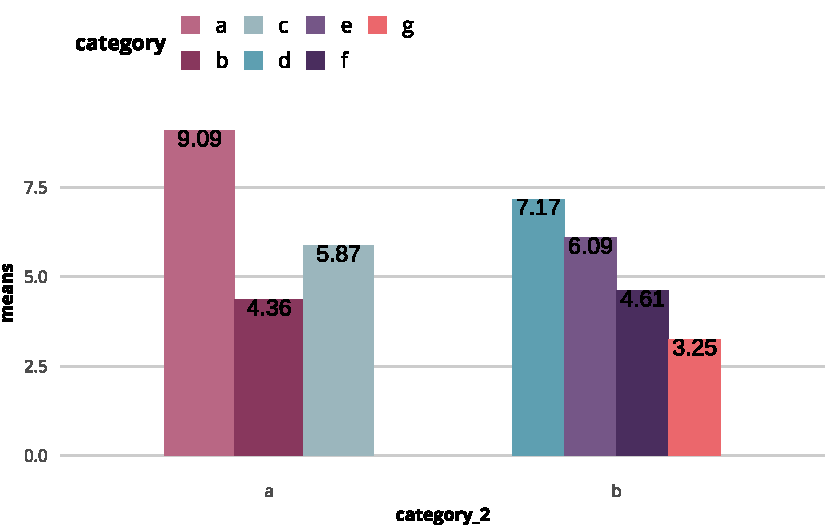
\includegraphics[keepaspectratio]{chart_types_files/figure-pdf/unnamed-chunk-3-1.pdf}}
\item
  long labels:

  Sometimes we might be working with very long labels for some
  categories. Those can be difficult to nicely render on a bar plot. 2
  ways to deal with this is either to flip coordinates that often makes
  the labels more readable or to wrap them so that they will have fixed
  maximum length on a single line. In case of flipping coordinates you
  will need to adjust the grid lines as well\\
  Option 1:

\begin{Shaded}
\begin{Highlighting}[]
\NormalTok{df\_long\_labs }\OtherTok{\textless{}{-}} \FunctionTok{data.frame}\NormalTok{(}
    \AttributeTok{item =} \FunctionTok{c}\NormalTok{(}\StringTok{"When I want to feel more positive emotion (such as joy or amusement), I change what I’m thinking about."}\NormalTok{,}
            \StringTok{"I keep my emotions to myself."}\NormalTok{,}
            \StringTok{"When I want to feel less negative emotion (such as sadness or anger), I change what I’m thinking about."}\NormalTok{,}
            \StringTok{"When I am feeling positive emotions, I am careful not to express them."}\NormalTok{),}
    \AttributeTok{mean =} \FunctionTok{c}\NormalTok{(}\FloatTok{4.54}\NormalTok{, }\FloatTok{2.34}\NormalTok{, }\FloatTok{6.44}\NormalTok{, }\FloatTok{3.55}\NormalTok{),}
    \AttributeTok{sd =} \FunctionTok{c}\NormalTok{(}\FloatTok{0.67}\NormalTok{, }\FloatTok{1.23}\NormalTok{, }\FloatTok{1.12}\NormalTok{, }\FloatTok{0.89}\NormalTok{)}
\NormalTok{)}

\NormalTok{df\_long\_labs }\SpecialCharTok{\%\textgreater{}\%}
\FunctionTok{ggplot}\NormalTok{(}\FunctionTok{aes}\NormalTok{(}\AttributeTok{x =}\NormalTok{ item, }\AttributeTok{y =}\NormalTok{ mean)) }\SpecialCharTok{+}
\FunctionTok{geom\_col}\NormalTok{(}\AttributeTok{fill =}\NormalTok{ cbu\_cat\_2[}\DecValTok{2}\NormalTok{], }\AttributeTok{width =}\NormalTok{ .}\DecValTok{6}\NormalTok{) }\SpecialCharTok{+}
\FunctionTok{geom\_text}\NormalTok{(}\FunctionTok{aes}\NormalTok{(}\AttributeTok{label =}\NormalTok{ mean), }\AttributeTok{nudge\_y =}\NormalTok{ .}\DecValTok{5}\NormalTok{) }\SpecialCharTok{+}
\FunctionTok{coord\_flip}\NormalTok{() }\SpecialCharTok{+}
\FunctionTok{theme\_cbu}\NormalTok{() }\SpecialCharTok{+}
\FunctionTok{theme}\NormalTok{(}\AttributeTok{panel.grid.major.y =} \FunctionTok{element\_blank}\NormalTok{(),}
     \AttributeTok{panel.grid.major.x =} \FunctionTok{element\_line}\NormalTok{(}\AttributeTok{color =} \StringTok{"grey80"}\NormalTok{, }\AttributeTok{linewidth =}\NormalTok{ .}\DecValTok{5}\NormalTok{))}
\end{Highlighting}
\end{Shaded}

  \pandocbounded{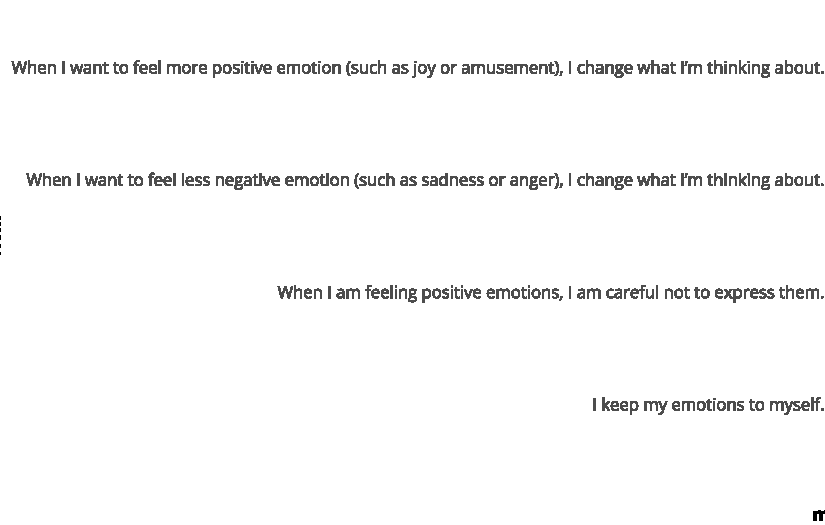
\includegraphics[keepaspectratio]{chart_types_files/figure-pdf/unnamed-chunk-4-1.pdf}}

  \hfill\break
  Option 2:

\begin{Shaded}
\begin{Highlighting}[]
\NormalTok{df\_long\_labs }\OtherTok{\textless{}{-}} \FunctionTok{data.frame}\NormalTok{(}
    \AttributeTok{item =} \FunctionTok{c}\NormalTok{(}\StringTok{"When I want to feel more positive emotion (such as joy or amusement), I change what I’m thinking about."}\NormalTok{,}
            \StringTok{"I keep my emotions to myself."}\NormalTok{,}
            \StringTok{"When I want to feel less negative emotion (such as sadness or anger), I change what I’m thinking about."}\NormalTok{,}
            \StringTok{"When I am feeling positive emotions, I am careful not to express them."}\NormalTok{),}
    \AttributeTok{mean =} \FunctionTok{c}\NormalTok{(}\FloatTok{4.54}\NormalTok{, }\FloatTok{2.34}\NormalTok{, }\FloatTok{6.44}\NormalTok{, }\FloatTok{3.55}\NormalTok{),}
    \AttributeTok{sd =} \FunctionTok{c}\NormalTok{(}\FloatTok{0.67}\NormalTok{, }\FloatTok{1.23}\NormalTok{, }\FloatTok{1.12}\NormalTok{, }\FloatTok{0.89}\NormalTok{)}
\NormalTok{)}

\NormalTok{df\_long\_labs }\SpecialCharTok{\%\textgreater{}\%}
\FunctionTok{ggplot}\NormalTok{(}\FunctionTok{aes}\NormalTok{(}\AttributeTok{x =} \FunctionTok{str\_wrap}\NormalTok{(item, }\DecValTok{40}\NormalTok{), }\AttributeTok{y =}\NormalTok{ mean)) }\SpecialCharTok{+}
\FunctionTok{geom\_col}\NormalTok{(}\AttributeTok{fill =}\NormalTok{ cbu\_cat\_2[}\DecValTok{2}\NormalTok{], }\AttributeTok{width =}\NormalTok{ .}\DecValTok{6}\NormalTok{) }\SpecialCharTok{+}
\FunctionTok{geom\_text}\NormalTok{(}\FunctionTok{aes}\NormalTok{(}\AttributeTok{label =}\NormalTok{ mean), }\AttributeTok{nudge\_y =}\NormalTok{ .}\DecValTok{5}\NormalTok{) }\SpecialCharTok{+}
\FunctionTok{coord\_flip}\NormalTok{() }\SpecialCharTok{+}
\FunctionTok{theme\_cbu}\NormalTok{() }\SpecialCharTok{+}
\FunctionTok{theme}\NormalTok{(}\AttributeTok{panel.grid.major.y =} \FunctionTok{element\_blank}\NormalTok{(),}
     \AttributeTok{panel.grid.major.x =} \FunctionTok{element\_line}\NormalTok{(}\AttributeTok{color =} \StringTok{"grey80"}\NormalTok{, }\AttributeTok{linewidth =}\NormalTok{ .}\DecValTok{5}\NormalTok{))}
\end{Highlighting}
\end{Shaded}

  \pandocbounded{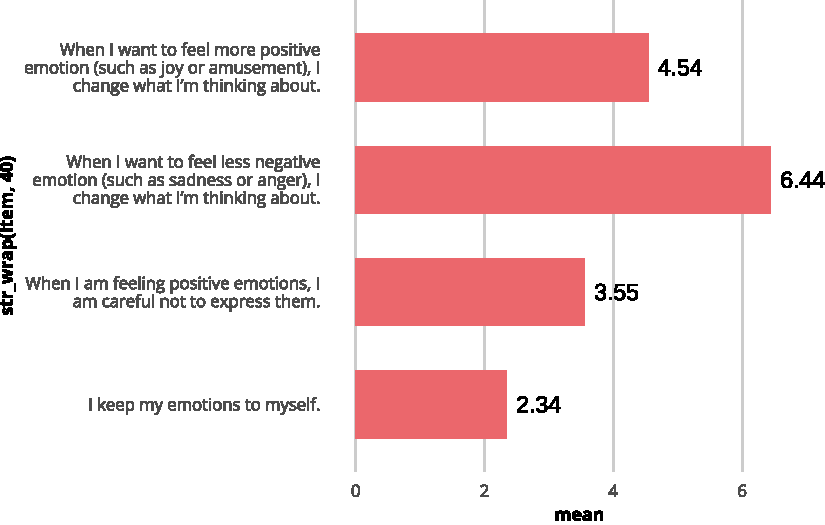
\includegraphics[keepaspectratio]{chart_types_files/figure-pdf/unnamed-chunk-5-1.pdf}}
\item
  adding errorbars:

\begin{Shaded}
\begin{Highlighting}[]
\NormalTok{df\_long\_labs }\SpecialCharTok{\%\textgreater{}\%}
\FunctionTok{ggplot}\NormalTok{(}\FunctionTok{aes}\NormalTok{(}\AttributeTok{x =}\NormalTok{ item, }\AttributeTok{y =}\NormalTok{ mean)) }\SpecialCharTok{+}
\FunctionTok{geom\_col}\NormalTok{(}\AttributeTok{fill =}\NormalTok{ cbu\_cat\_2[}\DecValTok{2}\NormalTok{], }\AttributeTok{width =}\NormalTok{ .}\DecValTok{6}\NormalTok{) }\SpecialCharTok{+}
\FunctionTok{geom\_errorbar}\NormalTok{(}\FunctionTok{aes}\NormalTok{(}\AttributeTok{x =}\NormalTok{ item, }\AttributeTok{ymin =}\NormalTok{ mean }\SpecialCharTok{{-}}\NormalTok{ sd, }\AttributeTok{ymax =}\NormalTok{ mean }\SpecialCharTok{+}\NormalTok{ sd), }\AttributeTok{width =}\NormalTok{ .}\DecValTok{2}\NormalTok{) }\SpecialCharTok{+}
\FunctionTok{theme\_cbu}\NormalTok{() }\SpecialCharTok{+}
\FunctionTok{theme}\NormalTok{(}\AttributeTok{panel.grid.major.y =} \FunctionTok{element\_blank}\NormalTok{(),}
     \AttributeTok{panel.grid.major.x =} \FunctionTok{element\_line}\NormalTok{(}\AttributeTok{color =} \StringTok{"grey80"}\NormalTok{, }\AttributeTok{linewidth =}\NormalTok{ .}\DecValTok{5}\NormalTok{))}
\end{Highlighting}
\end{Shaded}

  \pandocbounded{\includegraphics[keepaspectratio]{chart_types_files/figure-pdf/unnamed-chunk-6-1.pdf}}
\item
  some likert-scale related issues:

  \texttt{geom\_bar()} will always by default start the plots from 0.
  This is generally good behavior but in case of likert scale items we
  often want them to start from 1. The best way to adjsut this is via
  \texttt{coord\_cartesian()} and setting the ylim argument.

\begin{Shaded}
\begin{Highlighting}[]
\NormalTok{df\_long\_labs }\SpecialCharTok{\%\textgreater{}\%}
\FunctionTok{ggplot}\NormalTok{(}\FunctionTok{aes}\NormalTok{(}\AttributeTok{x =} \FunctionTok{str\_wrap}\NormalTok{(item, }\DecValTok{40}\NormalTok{), }\AttributeTok{y =}\NormalTok{ mean)) }\SpecialCharTok{+}
\FunctionTok{geom\_col}\NormalTok{(}\AttributeTok{fill =}\NormalTok{ cbu\_cat\_2[}\DecValTok{2}\NormalTok{], }\AttributeTok{width =}\NormalTok{ .}\DecValTok{6}\NormalTok{) }\SpecialCharTok{+}
\FunctionTok{geom\_text}\NormalTok{(}\FunctionTok{aes}\NormalTok{(}\AttributeTok{label =}\NormalTok{ mean), }\AttributeTok{nudge\_y =}\NormalTok{ .}\DecValTok{5}\NormalTok{) }\SpecialCharTok{+}
\FunctionTok{coord\_cartesian}\NormalTok{(}\AttributeTok{ylim=}\FunctionTok{c}\NormalTok{(}\DecValTok{1}\NormalTok{,}\DecValTok{7}\NormalTok{)) }\SpecialCharTok{+}
\FunctionTok{theme\_cbu}\NormalTok{()}
\end{Highlighting}
\end{Shaded}

  \pandocbounded{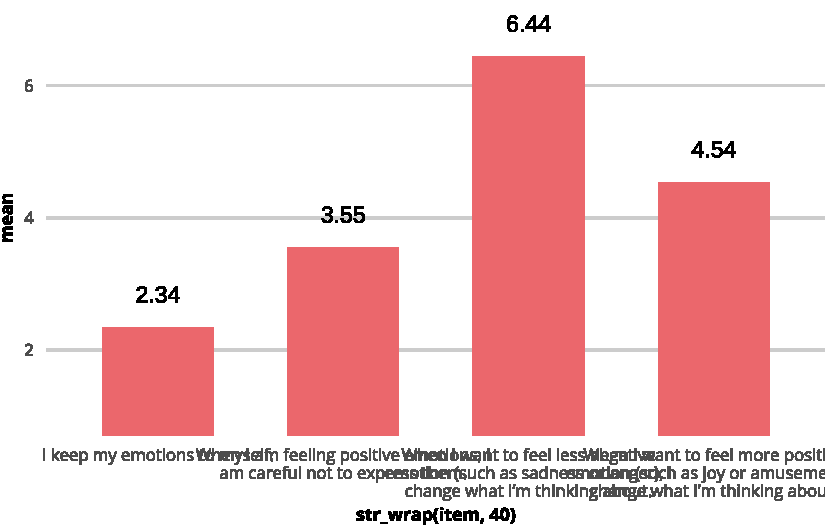
\includegraphics[keepaspectratio]{chart_types_files/figure-pdf/unnamed-chunk-7-1.pdf}}
\end{itemize}

\subsection{Filled bar charts}\label{filled-bar-charts}

We use those usually for displaying percentages (e.g.~distribution of
answers to a likert scale type question). Specific issues that often
arise with these kinds of plots are related to very small categories.
When trying to show text for those categories it can be difficult to get
non-overlappling and readable labels. Some ways to deal with this is to
collapse categories if possible or use \texttt{\{ggrepel\}} to push
text.

\begin{Shaded}
\begin{Highlighting}[]
\NormalTok{df\_cat }\OtherTok{\textless{}{-}} \FunctionTok{data.frame}\NormalTok{(}
    \AttributeTok{cat\_1 =} \FunctionTok{sample}\NormalTok{(letters[}\DecValTok{1}\SpecialCharTok{:}\DecValTok{4}\NormalTok{], }\FloatTok{1e3}\NormalTok{, }\AttributeTok{replace =} \ConstantTok{TRUE}\NormalTok{),}
    \AttributeTok{cat\_2 =} \FunctionTok{sample}\NormalTok{(letters[}\DecValTok{5}\SpecialCharTok{:}\DecValTok{7}\NormalTok{], }\FloatTok{1e3}\NormalTok{, }\AttributeTok{replace =} \ConstantTok{TRUE}\NormalTok{, }\AttributeTok{prob =} \FunctionTok{c}\NormalTok{(.}\DecValTok{01}\NormalTok{, .}\DecValTok{6}\NormalTok{, .}\DecValTok{39}\NormalTok{))}
\NormalTok{)}

\NormalTok{df\_cat }\SpecialCharTok{\%\textgreater{}\%}
\FunctionTok{count}\NormalTok{(cat\_1, cat\_2) }\SpecialCharTok{\%\textgreater{}\%}
\FunctionTok{group\_by}\NormalTok{(cat\_1) }\SpecialCharTok{\%\textgreater{}\%}
\FunctionTok{mutate}\NormalTok{(}\AttributeTok{perc =}\NormalTok{n}\SpecialCharTok{/}\FunctionTok{sum}\NormalTok{(n)) }\SpecialCharTok{\%\textgreater{}\%}
\FunctionTok{ggplot}\NormalTok{(}\FunctionTok{aes}\NormalTok{(}\AttributeTok{x =}\NormalTok{ cat\_1, }\AttributeTok{y =}\NormalTok{ perc, }\AttributeTok{fill =}\NormalTok{ cat\_2)) }\SpecialCharTok{+}
\FunctionTok{geom\_col}\NormalTok{(}\AttributeTok{width =}\NormalTok{ .}\DecValTok{6}\NormalTok{) }\SpecialCharTok{+}
\FunctionTok{geom\_text\_repel}\NormalTok{(}\FunctionTok{aes}\NormalTok{(}\AttributeTok{label =}\NormalTok{ scales}\SpecialCharTok{::}\FunctionTok{percent}\NormalTok{(perc)), }\AttributeTok{position =} \StringTok{"fill"}\NormalTok{, }\AttributeTok{direction =} \StringTok{"y"}\NormalTok{) }\SpecialCharTok{+}
\FunctionTok{scale\_fill\_manual}\NormalTok{(}\AttributeTok{values =}\NormalTok{ cbu\_cat\_2[}\FunctionTok{c}\NormalTok{(}\DecValTok{1}\NormalTok{,}\DecValTok{2}\NormalTok{,}\DecValTok{4}\NormalTok{)]) }\SpecialCharTok{+}
\FunctionTok{theme\_cbu}\NormalTok{()}
\end{Highlighting}
\end{Shaded}

\pandocbounded{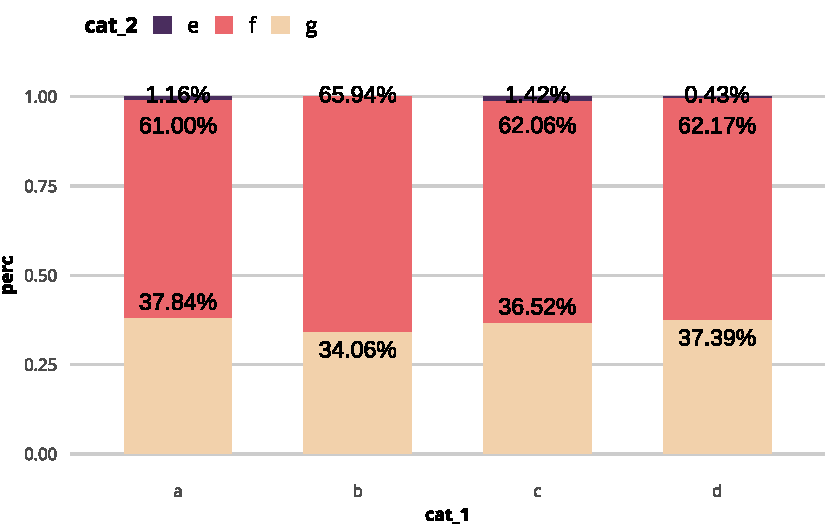
\includegraphics[keepaspectratio]{chart_types_files/figure-pdf/unnamed-chunk-8-1.pdf}}

\subsection{Line charts}\label{line-charts}

Line charts are usually best suited for showing changes in time. One
thing that sometimes comes up is a large number of lines that an make
the plot unreadable. If possible we can then try to highlight just one
(or a few) category and keep the rest in grey.

\begin{Shaded}
\begin{Highlighting}[]
\NormalTok{df\_lines }\OtherTok{\textless{}{-}} \FunctionTok{data.frame}\NormalTok{(}
    \AttributeTok{date =} \FunctionTok{rep}\NormalTok{(}\FunctionTok{c}\NormalTok{(}\DecValTok{2012}\NormalTok{,}\DecValTok{2013}\NormalTok{,}\DecValTok{2014}\NormalTok{,}\DecValTok{2015}\NormalTok{, }\DecValTok{2016}\NormalTok{), }\DecValTok{5}\NormalTok{),}
    \AttributeTok{category =} \FunctionTok{sort}\NormalTok{(}\FunctionTok{rep}\NormalTok{(letters[}\DecValTok{1}\SpecialCharTok{:}\DecValTok{5}\NormalTok{],}\DecValTok{5}\NormalTok{)),}
    \AttributeTok{value =} \FunctionTok{rnorm}\NormalTok{(}\DecValTok{25}\NormalTok{)}
\NormalTok{)}

\NormalTok{df\_lines }\SpecialCharTok{\%\textgreater{}\%}
\FunctionTok{ggplot}\NormalTok{(}\FunctionTok{aes}\NormalTok{(}\AttributeTok{x=}\NormalTok{date, }\AttributeTok{y =}\NormalTok{ value, }\AttributeTok{color =}\NormalTok{ category)) }\SpecialCharTok{+}
\FunctionTok{geom\_line}\NormalTok{(}\AttributeTok{linewidth =} \FloatTok{1.4}\NormalTok{) }\SpecialCharTok{+}
\FunctionTok{scale\_color\_manual}\NormalTok{(}\AttributeTok{values =}\NormalTok{ cbu\_cat\_2) }\SpecialCharTok{+}
\FunctionTok{theme\_cbu}\NormalTok{()}
\end{Highlighting}
\end{Shaded}

\pandocbounded{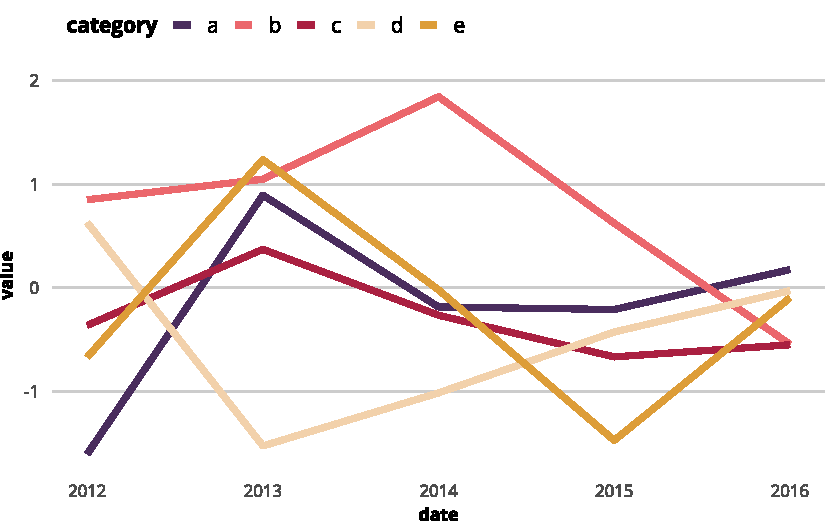
\includegraphics[keepaspectratio]{chart_types_files/figure-pdf/unnamed-chunk-9-1.pdf}}

\subsection{Scatterplots}\label{scatterplots}

Use cases are pretty obvious. The thing to remember is to deal with
overlapping points either by setting transparency, using
\texttt{geom\_count()} or adding jitter.

\begin{Shaded}
\begin{Highlighting}[]
\NormalTok{df\_scatter }\OtherTok{\textless{}{-}} \FunctionTok{data.frame}\NormalTok{(}
    \AttributeTok{x =} \FunctionTok{rnorm}\NormalTok{(}\FloatTok{1e3}\NormalTok{, }\DecValTok{4}\NormalTok{, }\FloatTok{1.2}\NormalTok{),}
    \AttributeTok{x\_2 =} \FunctionTok{rnorm}\NormalTok{(}\FloatTok{1e3}\NormalTok{, }\FloatTok{1.2}\NormalTok{, }\FloatTok{1.7}\NormalTok{),}
    \AttributeTok{cat =} \FunctionTok{factor}\NormalTok{(}\FunctionTok{rbinom}\NormalTok{(}\FloatTok{1e3}\NormalTok{, }\DecValTok{1}\NormalTok{, .}\DecValTok{5}\NormalTok{))}
\NormalTok{)}

\NormalTok{df\_scatter}\SpecialCharTok{$}\NormalTok{y }\OtherTok{\textless{}{-}} \FunctionTok{rnorm}\NormalTok{(}\FloatTok{1e3}\NormalTok{, }\DecValTok{2} \SpecialCharTok{+}\NormalTok{ .}\DecValTok{5}\SpecialCharTok{*}\NormalTok{df\_scatter}\SpecialCharTok{$}\NormalTok{x }\SpecialCharTok{{-}}\NormalTok{ .}\DecValTok{8}\SpecialCharTok{*}\NormalTok{df\_scatter}\SpecialCharTok{$}\NormalTok{x\_2 }\SpecialCharTok{+}\NormalTok{ .}\DecValTok{5}\SpecialCharTok{*}\NormalTok{df\_scatter}\SpecialCharTok{$}\NormalTok{x}\SpecialCharTok{*}\NormalTok{df\_scatter}\SpecialCharTok{$}\NormalTok{x\_2, }\FloatTok{1.4}\NormalTok{)}

\NormalTok{df\_scatter }\SpecialCharTok{\%\textgreater{}\%}
\FunctionTok{ggplot}\NormalTok{(}\FunctionTok{aes}\NormalTok{(}\AttributeTok{x =}\NormalTok{ x, }\AttributeTok{y =}\NormalTok{ y, }\AttributeTok{color =}\NormalTok{ cat)) }\SpecialCharTok{+}
\FunctionTok{geom\_count}\NormalTok{(}\AttributeTok{alpha =}\NormalTok{ .}\DecValTok{3}\NormalTok{) }\SpecialCharTok{+}
\FunctionTok{scale\_color\_manual}\NormalTok{(}\AttributeTok{values =}\NormalTok{ cbu\_cat\_2) }\SpecialCharTok{+}
\FunctionTok{theme\_cbu}\NormalTok{()}
\end{Highlighting}
\end{Shaded}

\pandocbounded{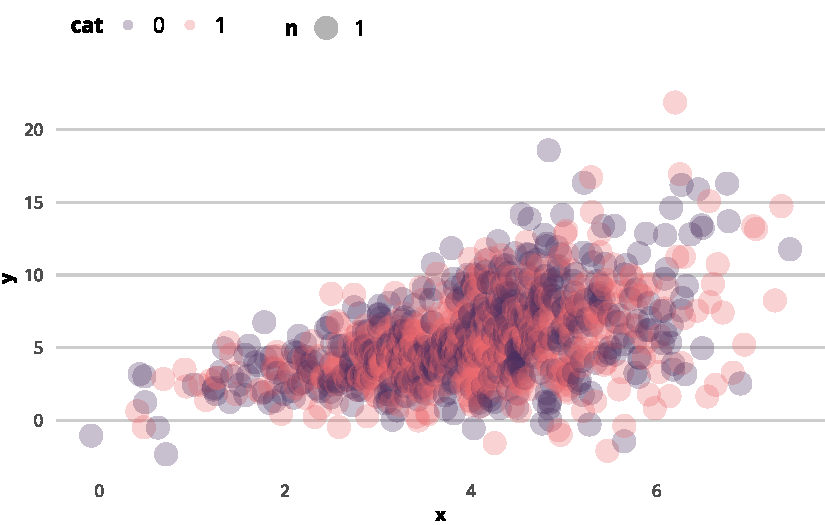
\includegraphics[keepaspectratio]{chart_types_files/figure-pdf/unnamed-chunk-10-1.pdf}}

\begin{itemize}
\item
  dealing with overplotting
\item
  Too many points -\textgreater{} go for geom\_count?
\item
  remember about reference line - geom\_point will happily start the y
  axis from a number different from 0 or 1
\end{itemize}

\subsection{Line-of-best-fit charts}\label{line-of-best-fit-charts}

This in general refers to plots that show some kind of regression-like
line of best fit, be it from a GLM, LOESS, GAM etc. Three things to
remember about with these kinds of plots is to work with the model
itself when plotting (rather than raw data), make sure a proper
interpretation is provided and try to include uncertainty.

\begin{Shaded}
\begin{Highlighting}[]
\FunctionTok{library}\NormalTok{(marginaleffects)}
\FunctionTok{library}\NormalTok{(splines)}
\NormalTok{fit\_df }\OtherTok{\textless{}{-}} \FunctionTok{data.frame}\NormalTok{(}
    \AttributeTok{x =} \FunctionTok{rnorm}\NormalTok{(}\FloatTok{1e3}\NormalTok{, }\FloatTok{3.4}\NormalTok{, }\FloatTok{1.2}\NormalTok{)}
\NormalTok{)}
\NormalTok{fit\_df}\SpecialCharTok{$}\NormalTok{y }\OtherTok{\textless{}{-}} \FunctionTok{rnorm}\NormalTok{(}\FloatTok{1e3}\NormalTok{, }\DecValTok{1} \SpecialCharTok{+} \DecValTok{3}\SpecialCharTok{*}\FunctionTok{sin}\NormalTok{(fit\_df}\SpecialCharTok{$}\NormalTok{x) }\SpecialCharTok{{-}} \FloatTok{1.2}\SpecialCharTok{*}\FunctionTok{cos}\NormalTok{(fit\_df}\SpecialCharTok{$}\NormalTok{x) }\SpecialCharTok{+}\NormalTok{ .}\DecValTok{2}\SpecialCharTok{*}\NormalTok{fit\_df}\SpecialCharTok{$}\NormalTok{x}\SpecialCharTok{\^{}}\DecValTok{2}\NormalTok{, .}\DecValTok{6}\NormalTok{)}

\NormalTok{model\_fit }\OtherTok{\textless{}{-}} \FunctionTok{lm}\NormalTok{(y }\SpecialCharTok{\textasciitilde{}} \FunctionTok{ns}\NormalTok{(x, }\DecValTok{3}\NormalTok{), fit\_df)}

\FunctionTok{plot\_predictions}\NormalTok{(model\_fit, }\AttributeTok{condition =} \StringTok{"x"}\NormalTok{) }\SpecialCharTok{+}
\FunctionTok{geom\_point}\NormalTok{(}\AttributeTok{data =}\NormalTok{ fit\_df, }\FunctionTok{aes}\NormalTok{(}\AttributeTok{x =}\NormalTok{ x, }\AttributeTok{y =}\NormalTok{ y), }\AttributeTok{alpha =}\NormalTok{ .}\DecValTok{3}\NormalTok{) }\SpecialCharTok{+}
\FunctionTok{theme\_cbu}\NormalTok{()}
\end{Highlighting}
\end{Shaded}

\pandocbounded{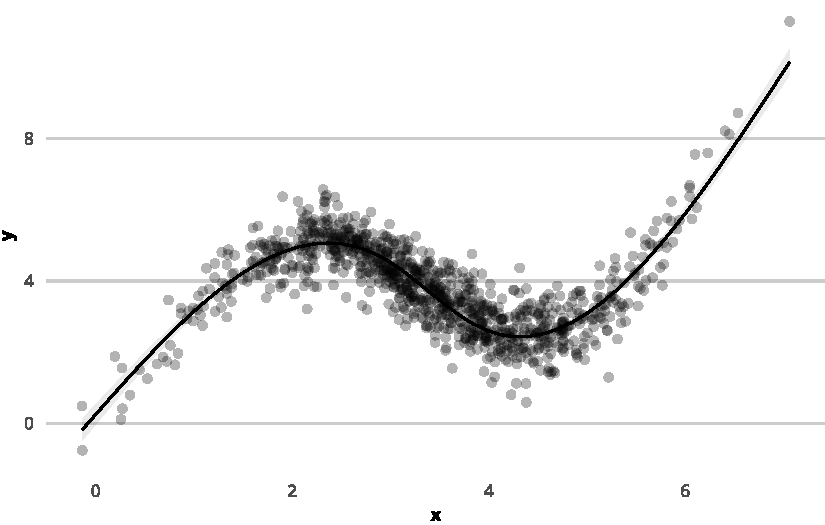
\includegraphics[keepaspectratio]{chart_types_files/figure-pdf/unnamed-chunk-11-1.pdf}}

\subsection{Correlation plots?}\label{correlation-plots}

Quite commonly cbu reports graphically display correlations. One way
which was commonly used was to make bar plots with heights of bar
representing strength of the correlation. Some alternatives include
dumbbell charts that use points instead of bars

\begin{Shaded}
\begin{Highlighting}[]
\NormalTok{cor\_df }\OtherTok{\textless{}{-}} \FunctionTok{data.frame}\NormalTok{(}
    \AttributeTok{cor =} \FunctionTok{c}\NormalTok{(.}\DecValTok{44}\NormalTok{, .}\DecValTok{34}\NormalTok{, .}\DecValTok{21}\NormalTok{, .}\DecValTok{13}\NormalTok{, .}\DecValTok{11}\NormalTok{, }\SpecialCharTok{{-}}\NormalTok{.}\DecValTok{23}\NormalTok{),}
    \AttributeTok{var =} \FunctionTok{sort}\NormalTok{(}\FunctionTok{rep}\NormalTok{(}\FunctionTok{c}\NormalTok{(}\StringTok{"SDO"}\NormalTok{, }\StringTok{"RWA"}\NormalTok{, }\StringTok{"Identification"}\NormalTok{), }\DecValTok{2}\NormalTok{)),}
    \AttributeTok{group =} \FunctionTok{rep}\NormalTok{(}\FunctionTok{c}\NormalTok{(}\StringTok{"group a"}\NormalTok{, }\StringTok{"group b"}\NormalTok{), }\DecValTok{3}\NormalTok{)}
\NormalTok{)}

\NormalTok{cor\_df }\SpecialCharTok{\%\textgreater{}\%}
\FunctionTok{ggplot}\NormalTok{(}\FunctionTok{aes}\NormalTok{(}\AttributeTok{y =}\NormalTok{ cor, }\AttributeTok{x =}\NormalTok{ var, }\AttributeTok{fill =}\NormalTok{ group)) }\SpecialCharTok{+}
\FunctionTok{geom\_col}\NormalTok{(}\AttributeTok{position =} \FunctionTok{position\_dodge}\NormalTok{(}\AttributeTok{width =}\NormalTok{ .}\DecValTok{9}\NormalTok{)) }\SpecialCharTok{+}
\FunctionTok{geom\_text}\NormalTok{(}\FunctionTok{aes}\NormalTok{(}\AttributeTok{label =}\NormalTok{ cor), }\AttributeTok{position =} \FunctionTok{position\_dodge}\NormalTok{(}\AttributeTok{width =}\NormalTok{ .}\DecValTok{9}\NormalTok{), }\AttributeTok{size =} \DecValTok{5}\NormalTok{) }\SpecialCharTok{+}
\FunctionTok{coord\_flip}\NormalTok{() }\SpecialCharTok{+}
\FunctionTok{scale\_fill\_manual}\NormalTok{(}\AttributeTok{values =}\NormalTok{ cbu\_cat\_1) }\SpecialCharTok{+}
\FunctionTok{theme\_cbu}\NormalTok{() }\SpecialCharTok{+}
\FunctionTok{theme}\NormalTok{(}\AttributeTok{panel.grid.major.y =} \FunctionTok{element\_blank}\NormalTok{(),}
     \AttributeTok{panel.grid.major.x =} \FunctionTok{element\_line}\NormalTok{(}\AttributeTok{color =} \StringTok{"grey80"}\NormalTok{))}
\end{Highlighting}
\end{Shaded}

\pandocbounded{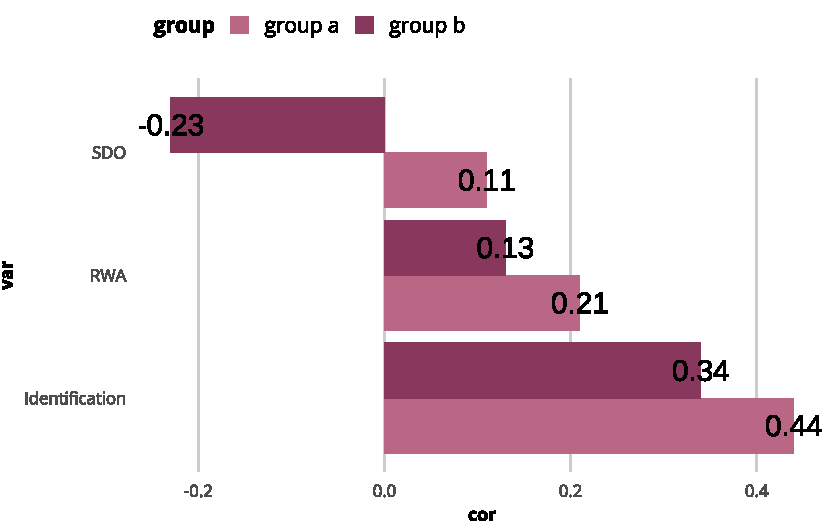
\includegraphics[keepaspectratio]{chart_types_files/figure-pdf/unnamed-chunk-12-1.pdf}}

\subsection{Dumbbell charts}\label{dumbbell-charts}

Dumbell charts are good for comparing changes or categories

\begin{Shaded}
\begin{Highlighting}[]
\NormalTok{df\_dc }\OtherTok{\textless{}{-}} \FunctionTok{data.frame}\NormalTok{(}
    \AttributeTok{x =} \FunctionTok{c}\NormalTok{(}\DecValTok{2020}\NormalTok{, }\DecValTok{2024}\NormalTok{, }\DecValTok{2020}\NormalTok{, }\DecValTok{2024}\NormalTok{, }\DecValTok{2020}\NormalTok{, }\DecValTok{2024}\NormalTok{),}
    \AttributeTok{y =} \FunctionTok{c}\NormalTok{(}\FloatTok{5.6}\NormalTok{, }\FloatTok{3.4}\NormalTok{, }\FloatTok{2.5}\NormalTok{, }\FloatTok{5.1}\NormalTok{, }\FloatTok{4.3}\NormalTok{, }\FloatTok{4.8}\NormalTok{),}
    \AttributeTok{cat =} \FunctionTok{c}\NormalTok{(}\StringTok{"a"}\NormalTok{, }\StringTok{"a"}\NormalTok{, }\StringTok{"b"}\NormalTok{, }\StringTok{"b"}\NormalTok{, }\StringTok{"c"}\NormalTok{, }\StringTok{"c"}\NormalTok{)}
\NormalTok{)}

\NormalTok{df\_dc }\SpecialCharTok{\%\textgreater{}\%}
\FunctionTok{ggplot}\NormalTok{(}\FunctionTok{aes}\NormalTok{(}\AttributeTok{x =}\NormalTok{ cat, }\AttributeTok{y =}\NormalTok{ y, }\AttributeTok{color =} \FunctionTok{factor}\NormalTok{(x))) }\SpecialCharTok{+}
\FunctionTok{geom\_line}\NormalTok{(}\FunctionTok{aes}\NormalTok{(}\AttributeTok{group =}\NormalTok{ cat), }\AttributeTok{color =} \StringTok{"grey60"}\NormalTok{) }\SpecialCharTok{+}
\FunctionTok{geom\_point}\NormalTok{(}\AttributeTok{size =} \DecValTok{3}\NormalTok{) }\SpecialCharTok{+}
\FunctionTok{geom\_text}\NormalTok{(}\FunctionTok{aes}\NormalTok{(}\AttributeTok{label =}\NormalTok{ y), }\AttributeTok{nudge\_x =}\NormalTok{ .}\DecValTok{2}\NormalTok{) }\SpecialCharTok{+}
\FunctionTok{scale\_color\_manual}\NormalTok{(}\AttributeTok{values =}\NormalTok{ cbu\_cat\_1) }\SpecialCharTok{+}
\FunctionTok{coord\_flip}\NormalTok{() }\SpecialCharTok{+}
\FunctionTok{theme\_cbu}\NormalTok{() }\SpecialCharTok{+}
\FunctionTok{theme}\NormalTok{(}\AttributeTok{panel.grid.major.y =} \FunctionTok{element\_blank}\NormalTok{(),}
     \AttributeTok{panel.grid.major.x =} \FunctionTok{element\_line}\NormalTok{(}\AttributeTok{color =} \StringTok{"grey80"}\NormalTok{))}
\end{Highlighting}
\end{Shaded}

\pandocbounded{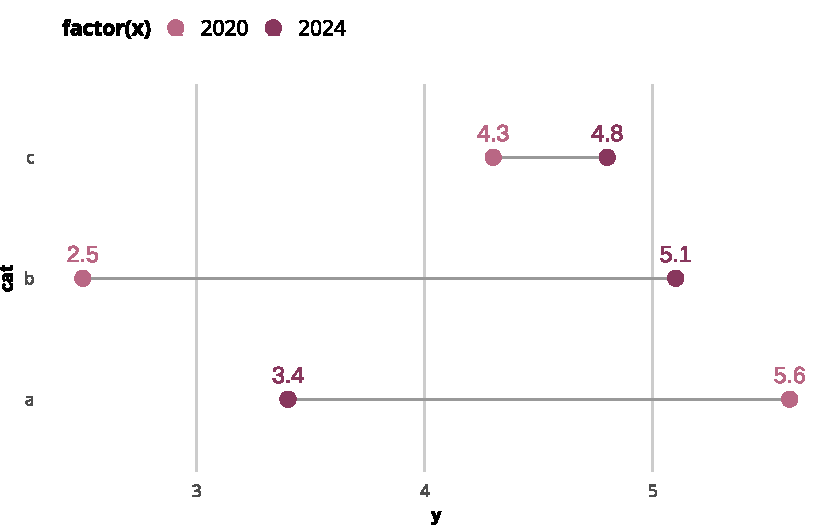
\includegraphics[keepaspectratio]{chart_types_files/figure-pdf/unnamed-chunk-13-1.pdf}}

\subsection{Waffle charts}\label{waffle-charts}

Waffle charts can be used as alternative to bar charts for displaying
counts or percentages. Preferrably they should also have numbers shown.

\begin{Shaded}
\begin{Highlighting}[]
\FunctionTok{library}\NormalTok{(waffle)}

\NormalTok{df\_cat }\SpecialCharTok{\%\textgreater{}\%}
\FunctionTok{count}\NormalTok{(cat\_1, cat\_2) }\SpecialCharTok{\%\textgreater{}\%}
\FunctionTok{ggplot}\NormalTok{(}
    \FunctionTok{aes}\NormalTok{(}\AttributeTok{fill =}\NormalTok{ cat\_1, }\AttributeTok{values =}\NormalTok{ n)}
\NormalTok{  ) }\SpecialCharTok{+}
  \FunctionTok{geom\_waffle}\NormalTok{(}
    \AttributeTok{n\_rows =} \DecValTok{20}\NormalTok{,}
    \AttributeTok{size =} \FloatTok{0.33}\NormalTok{, }
    \AttributeTok{colour =} \StringTok{"white"}\NormalTok{,}
    \AttributeTok{flip =} \ConstantTok{TRUE}
\NormalTok{  ) }\SpecialCharTok{+}
  \FunctionTok{scale\_fill\_manual}\NormalTok{(}
    \AttributeTok{name =} \ConstantTok{NULL}\NormalTok{,}
    \AttributeTok{values =}\NormalTok{ cbu\_cat\_2}
\NormalTok{  ) }\SpecialCharTok{+}
  \FunctionTok{facet\_wrap}\NormalTok{(}\SpecialCharTok{\textasciitilde{}}\NormalTok{cat\_2, }\AttributeTok{nrow =} \DecValTok{1}\NormalTok{) }\SpecialCharTok{+}
  \FunctionTok{coord\_equal}\NormalTok{() }\SpecialCharTok{+}
  \FunctionTok{theme\_enhance\_waffle}\NormalTok{() }\SpecialCharTok{+}
  \FunctionTok{theme\_cbu}\NormalTok{()}
\end{Highlighting}
\end{Shaded}

\pandocbounded{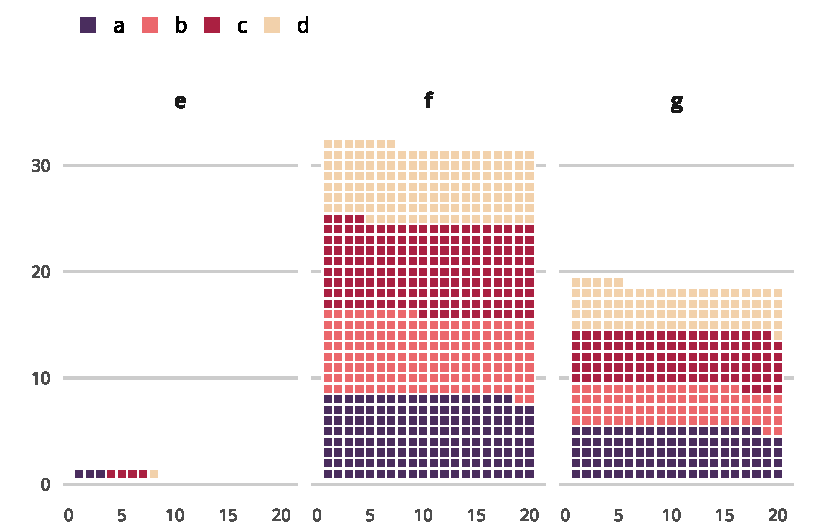
\includegraphics[keepaspectratio]{chart_types_files/figure-pdf/unnamed-chunk-14-1.pdf}}

\subsection{Pie charts}\label{pie-charts}

just no. Make a bar chart. Or a waffle chart

\subsection{Showing statistical
models}\label{showing-statistical-models}

One additional type of charts that sometimes appears in the reports are
path diagrams showing path/SEM models. Unfortunately there isn't really
any good package for displaying path diagrams. IF you really want to
make it in R you can use \texttt{\{ggdag\}} but all the nodes, positions
and text has to be coded manually.

You can make such diagrams in Figma, diagram.net or Power Point. If you
do that remember to use Open Sans font, preferrably size 12 or 14.

\bookmarksetup{startatroot}

\chapter{}\label{section}

What this tutorial has to include:

\begin{enumerate}
\def\labelenumi{\arabic{enumi}.}
\tightlist
\item
  General introduction to quarto?
\item
  Overview of the format and its tech stack:

  \begin{enumerate}
  \def\labelenumii{\arabic{enumii}.}
  \tightlist
  \item
    quarto to write so we work in markdown
  \item
    typst to render to pdf. DO NOT TOUCH
  \item
    Zotero for citations
  \item
    R/python/julia for calculations. Preferably R
  \end{enumerate}
\item
  Walkthrough making a report

  \begin{enumerate}
  \def\labelenumii{\arabic{enumii}.}
  \tightlist
  \item
    Writing regular text
  \item
    footnotes
  \item
    Headings: we use level 4 headings for sections
  \item
    Making tables
  \item
    Making plots
  \item
    References:

    \begin{enumerate}
    \def\labelenumiii{\arabic{enumiii}.}
    \tightlist
    \item
      Zotero
    \item
      referencing tables and plots
    \end{enumerate}
  \end{enumerate}
\end{enumerate}

\bookmarksetup{startatroot}

\chapter{Summary}\label{summary}

In summary, this book has no content whatsoever.

\begin{Shaded}
\begin{Highlighting}[]
\DecValTok{1} \SpecialCharTok{+} \DecValTok{1}
\end{Highlighting}
\end{Shaded}

\begin{verbatim}
[1] 2
\end{verbatim}

\bookmarksetup{startatroot}

\chapter*{References}\label{references}
\addcontentsline{toc}{chapter}{References}

\markboth{References}{References}

\phantomsection\label{refs}
\begin{CSLReferences}{0}{1}
\end{CSLReferences}




\end{document}
